% % part: 微分方程
% % chap: 常微分方程


% % 图片大小要调整;
% % MATALB图片不同曲线不能用不同颜色标识,要用线形标识;

% \documentclass[UTF8]{ctexbook}

% \ctexset{
%     part/number = \chinese{part}
% }
% \usepackage{multirow}
% \usepackage{amsmath}% ams 数学公式
% \usepackage{amsfonts}% ams 数学字体
% \usepackage{bbm}%重影字体
% \usepackage{amssymb,latexsym}% ams 数学符号与LaTeX数学符号
% \usepackage{mathrsfs}% 花式符号
% \usepackage{ntheorem}%定理、定义、证明
%     \theoremstyle{nonumberplain}
%     \theoremheaderfont{\bfseries}
%     \theorembodyfont{\normalfont}
%     \theoremsymbol{$\square$}
%     \newtheorem{Proof}{\hskip 2em 证明}
%     \newtheorem{theorem}{\hspace{2em}定理}[chapter]
%     \newtheorem{definition}{\hspace{2em}定义}[chapter] % 如果没有章, 只有节, 把上面的[chapter]改成[section]
%     \newtheorem{axiom}[definition]{\hspace{2em}公理}
%     \newtheorem{lemma}[definition]{\hspace{2em}引理}
%     \newtheorem{proposition}[definition]{\hspace{2em}命题}
%     \newtheorem{corollary}[definition]{\hspace{2em}推论}
%     \newtheorem{remark}{\hspace{2em}注}[chapter] %类似地定义其他“题头”. 这里“注”的编号与定义、定理等是分开的
%     \newtheorem{Assumption}{\hspace{2em}假设}[chapter]

% %算法伪代码
% %http://blog.csdn.net/lwb102063/article/details/53046265
% \usepackage{algorithm}
% \usepackage{algorithmicx}
% \usepackage{algpseudocode}
%     \floatname{algorithm}{算法}
%     \renewcommand{\algorithmicrequire}{\textbf{输入:}}
%     \renewcommand{\algorithmicensure}{\textbf{输出:}}
% % 罗马数字:示例:\rom{2}
% \makeatletter
% \newcommand*{\rom}[1]{\expandafter\@slowromancap\romannumeral #1@}
% \makeatother

% \usepackage{enumerate}%itemiz环境。\begin{enumerate}[step 1][a)]可以使用 A,a,I,i,1 作为可选项产生 \Alph,\alph,\Roman,\roman,\arabic 的效果
% \usepackage{cite}%参考文献
%     \bibliographystyle{plain}
% \usepackage{extarrows}% 带参数的箭头
% \usepackage{hyperref}% 超链接
% \usepackage{pifont}%然后在正文输入\ding{172}~\ding{211}得到相应数字,要是要①就输入:\ding{172}②就输:\ding{173}
% %\usepackage[CJKbookmarks, colorlinks, bookmarksnumbered=true,pdfstartview=FitH,linkcolor=black,citecolor=black]{hyperref}%超链接的格式设置
% \hypersetup{
%     colorlinks=false,% 去掉超链接颜色
%     pdfborder=0 0 0% 取消超链接的边框
% }
% \usepackage{graphicx}% 图片管理
% \usepackage{caption}
% \usepackage{subcaption}%并排的图各有标题
% \graphicspath{{images/}}% 设置图片搜索路径
% \usepackage{float,varwidth}% 浮动体
% \usepackage{booktabs}% 三线表
% \usepackage{fancyhdr}% 页眉设置
% \usepackage{xcolor}% 颜色宏包
% \usepackage{colortbl}% 彩色表格
% \usepackage{listings}% 代码高亮
% \usepackage{caption}% 对标题进行控制,如让\caption标题的字体缩小一号,同时数字标签使用粗体可以用:\usepackage[font=small,labelfont=bf]{caption}
% \usepackage{xfrac,upgreek}%分别是行间公式如a/b的形式(将原来的命令\frac改成\sfrac)和希腊字体的宏包的
% \usepackage{mathtools}%lgathered和rgathered环境把公式向左向右对齐
% \usepackage{tabularx}%提供自动延伸的表列,(X列格式说明符),文字过长时可以自动转行
% \usepackage{longtable}%长表格
% \usepackage{enumitem}%enumerate宏包的升级
% \usepackage{harpoon}%数学公式的矢量
% \usepackage{bookmark}%目录的书签
% \renewcommand{\headwidth}{\textwidth}%图片并排,这个要列在所有宏包的后面
% \definecolor{codegreen}{rgb}{0,0.6,0}
% \definecolor{codegray}{rgb}{0.5,0.5,0.5}
% \definecolor{codepurple}{rgb}{0.58,0,0.82}
% \definecolor{backcolour}{rgb}{0.95,0.95,0.92}
% \lstset{
%     commentstyle=\color{codegreen},
%     keywordstyle=\color{magenta},
%     numberstyle=\tiny\color{codegray},
%     stringstyle=\color{codepurple},
%     basicstyle=\footnotesize,
%     breakatwhitespace=false,% 断行只在空格处
%     breaklines=true,% 自动断行
%     captionpos=b,% 标题位置
%     keepspaces=true,
%     numbers=left,
%     numbersep=5pt,
%     showspaces=false,
%     showstringspaces=false,
%     showtabs=false,% 显示
%     tabsize=2% TAB 被当作两个空格
% }
% \topmargin=0pt\oddsidemargin=0pt\evensidemargin=0pt
% \textwidth=16.5cm\textheight=23cm\raggedbottom%我这么设置是为了缩小页边距,满足有的文字无法转行
% \pagestyle{headings}%页眉为章节标题,无页脚
% \setlength{\abovecaptionskip}{10pt}
% \setlength{\belowcaptionskip}{-15pt}%图片表格的前后距离设置
% \CTEXsetup[format={\zihao{-3}\raggedright\bfseries}]{section}%设置节的格式

% \begin{document}
% \part{微分方程}\label{prt:de}
\chapter{常微分方程}\label{cha:ode}
\section{常微分方程建模}\label{sec:de-ode-modeling}
	\subsection{数学摆的微分方程}
		\label{sub:de-ode-modeling-pendulum}
		数学摆是质量为 $m$ 的物体 $M$ 系于一长为 $l$ 的线上,在重力的作用下沿圆周运动,如图(\ref{fig:单摆示意图})所示,求物体的运动方程。
		\par
		% \textcolor[rgb]{1.00,0.00,0.00}{todo:图片:单摆示意图}
		\begin{figure}[H]
		\centering
		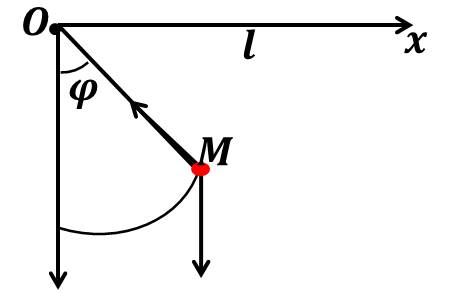
\includegraphics[width=4cm]{pendulum_sketch.jpg}% 图叫:单摆-示意图
		\caption{单摆示意图}
		\label{fig:单摆示意图}
		\end{figure}
		解:像一般分析的那样,先假设,再确定变量,然后是建立坐标系、受力分析,最终我们会有它的运动方程。
		\par
		假设1:质量为 $m$ 的物体 $M$ 仅受重力和拉力作用,忽略其它力;假设2:物体 $M$ 在初始点处的速度 $v$ 是 0;假设3:物体 $M$ 视为质点;假设4:物体初始位置在固定点水平右方(保持细线拉直);就此题来看,我们应建立二维坐标系,并且用极坐标系可能更方便一些,因为我们有了极径 $l$。
		\par
		建系:以线端点 $o$ 为坐标原点,水平向右方向为 $x$ 轴正向,竖直向下(重力方向)为 $y$ 轴方向,建立平面直角坐标系 $xoy$.
		\par
		设置变量:设线长为 $l$ ,线与 $y$ 轴夹角为 $\varphi$,物体 $M$ 的质量为 $m$,初始时刻为 $t_0$ (不妨设物体 $M$ 的坐标为 $(x,y)$, 其实不必要)。
		\par
		受力分析:物体 $M$ 的受力分析示意图如图(\ref{fig:单摆受力分析示意图})所示,我们要在受力分析的基础上,确定各时刻 $t$ 的 $\varphi$ 的大小,即确定曲线 $\varphi(t)$。
		 \begin{figure}[H]
		\centering
		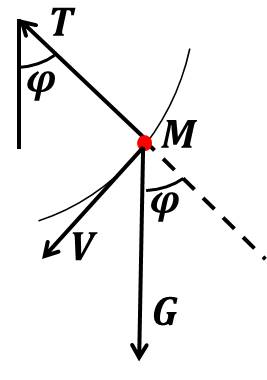
\includegraphics[height=3cm]{images/pendulum_sketch_force_analysis.jpg}% 图叫:单摆-受力分析
		\caption{单摆受力分析}
		\label{fig:单摆受力分析示意图}
		\end{figure}
		其在 $M$ 点处受重力 $G$ 和拉力 $T$ 的作用,速度为 $v$,有
		\begin{align*}
			&G = mg \\
			&G \cos{\varphi} = T
		\end{align*}
		所以是 $G\sin{\varphi}$ 提供加速度,故
		\[
			\dot{v} = G \cdot \sin{\varphi} / m = g \cdot \sin{\varphi}
		\]
		而由运动方程 $v = \omega \cdot l$,我们有
		\[
			v = l \cdot \dot{\varphi} \quad (\varphi(t_0) = \varphi_0)
		\]
		所以,可以确定最终的运动方程为
		\begin{align*}
			\left\{
				\begin{aligned}
				&l \cdot \ddot{\varphi} = g \cdot \sin{\varphi}\\
				&\ddot{\varphi} = g/l \cdot \sin{\varphi}
				\end{aligned}
			\right.
		\end{align*}
		或者写为
		\par
		\begin{equation}
			\frac{\mathrm{d}^2\varphi}{\mathrm{d}t^2} = g/l \cdot \sin{\varphi}
			\label{eq:摆的二阶微分方程}
		\end{equation}
		\par
		给定初始条件:$\varphi(t_0) = \varphi_0$,其中:$t_0$ 是初始时间,$\varphi$ 为初始(刚开始下落时)的夹角大小。此时,我们的目标就变为求一个 $\varphi(t)$ 函数,$\varphi(t)$ 应满足方程(\ref{eq:摆的二阶微分方程})以及 $\varphi(t_0) = \varphi_0$ 的初始条件。
	\subsection{传染病模型}
		\label{sub:sub:de-ode-modeling-sir}
		第一次参加建模是 2014 年小美赛,当时要处理的问题正是传染病“埃博拉”。经过查找文献,找到了 SIR 模型,懵懵懂懂的将模型改进为 SIRAB(当时实在不知道该用个啥样的名字),但建立完 SIRAB 之后,问题也随之而来,这是个什么模型,怎么解?
		\par
		对于传染病而言,我们更关心的是随着时间 $t$ 的增长,感染的人数是如何变化的,如何对传染病进行控制,所以至少我们会有下面的图(\ref{fig:感染人数增长示意图})
		% \textcolor[rgb]{1.00,0.00,0.00}{todo:图片:感染人数增长示意图}
		\begin{figure}[H]
		\centering
		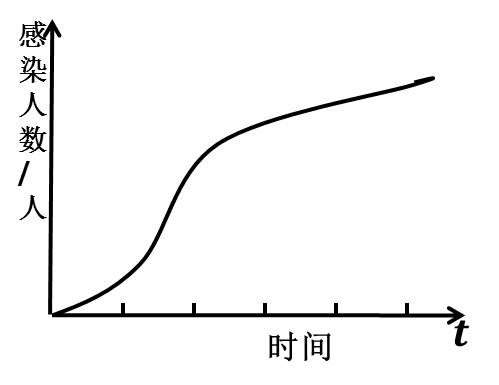
\includegraphics[width=4cm]{images/Infection_increased_schematic_diagram.jpg}% 图叫:单摆-示意图
		\caption{感染人数增长示意图}
		\label{fig:感染人数增长示意图}
		\end{figure}
		\par
		我们不妨将其离散化,问题是:如果我们知道了 $t$ 时刻的感染人数,那 $t + 1$ 时刻的人数会是多少。
		我们考虑一个地区$A$,$A$在$t$时刻共有$N(t)$个人,如果地区$A$不是封闭的话,$t+1$时刻$N(t)$可能增加也可能减少。为了简单,我们假设地区$A$的人口总数恒为$N$。如果我们知道了$A$地区$t$时刻的染病人数,如何求$t+1$时刻的染病人数?设染病人数为$I(t)$,那么未感染人数就变为了$N-I(t)$,假设未感染的人群都是易感染者,记为$S(t)$(当然,实际情况可能是未感染人群中部分人已经有免疫能力了,那么他就不易变为感染者)。我们建立下面的传染病SI模型
		\begin{align*}
			 \left\{
				 \begin{aligned}
					 &I(t+\Delta t) = I(t) + \alpha S(t) \Delta t\\
					 &S(t+\Delta t) = S(t) - \alpha S(t) \Delta t\\
					 &I(t) + S(t) = I(t+1)+S(t+1) = N
				 \end{aligned}
			 \right.
		\end{align*}
		其中:$\alpha$为单位时间内未感染者变为感染者的可能,记为发病率。
		将上式转化为
		\begin{align*}
			 \left\{
				 \begin{aligned}
					 &\dot{I}(t) = \alpha S(t) \approx \Delta I(t)\\
					 &\dot{S}(t) = - \alpha S(t) \approx \Delta S(t)\\
					 &I(t) + S(t) = N
				 \end{aligned}
			 \right.
		\end{align*}
		为方便理解,$\dot{I}(t) \approx \Delta I(t)$记为$t$时刻传染者新增的人数,$\alpha S(t)$为$t$时刻未感染者$S(t)$转化为感染者的人数。
		\par
		对于上面的SI模型,我们有许多可以改进方法,比如,我们可以做如下改进:
		\par
		(1)前面,我们假设地区$A$在个时刻$t$内仅有两种人:感染者$I$和未感染者$S$。实际上,还可能有感染之后恢复的人,并且这类人不会再染病,我们记这类人为$R$,设染病者的恢复率为$\beta$,则$A$地区不同人群的人口转移如图(\ref{fig:SIR感染者转移示意图})所示
		\begin{figure}[H]
		\centering
		
\includegraphics[width=4cm]{images/SIR_Infection_transfer.jpg}
		\caption{SIR感染者转移示意图}
		\label{fig:SIR感染者转移示意图}
		\end{figure}
		由此可建立微分方程模型
		\begin{align*}
			 \left\{
				 \begin{aligned}
					 &\dot{I}(t) = \alpha S(t)- \beta I(t)\\
					 &\dot{S}(t) = - \alpha S(t)\\
					 &\dot{R}(t) = \beta I(t)\\
					 &I(t) + S(t) + R(t) = N
				 \end{aligned}
			 \right.
		\end{align*}
		(2)还有一种可能是:在$[t_0-t_1]$时间段内不存在$R$类人,在$t_1$时刻(疫苗到达时)出现了$R$类人。
		\par
		(3)我们还可以假设这个传染病是有潜伏期的,未感染者$S$先变为潜伏者$E$($E$不表现为发病),然后潜伏者才变为感染者$S$,其转移情况如图(\ref{fig:SIRE感染者转移示意图})所示
		\begin{figure}[H]
		\centering
		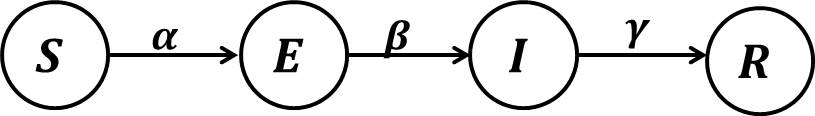
\includegraphics[width=4cm]{images/SIRE_Infection_transfer.jpg}
		\caption{SIRE感染者转移示意图}
		\label{fig:SIRE感染者转移示意图}
		\end{figure}
		% \textcolor[rgb]{1.00,0.00,0.00}{todo:图片:SIRE感染者转移示意图}\\
		(4)我们在来假设一部分感染者$S$死亡了,记死亡者为$D$,可以建立SEIRD传染病模型,其转移情况如图(\ref{fig:SEIRD感染者转移示意图})所示
		\begin{figure}[H]
		\centering
		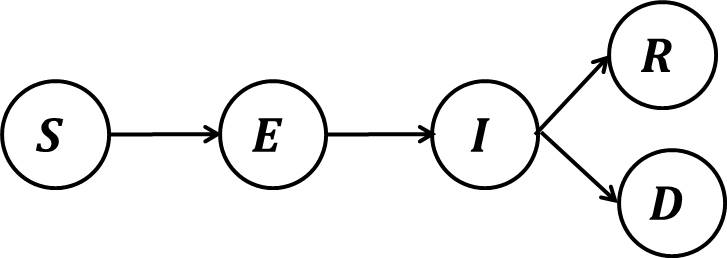
\includegraphics[width=4cm]{images/SEIRD_Infection_transfer.jpg}
		\caption{SEIRD感染者转移示意图}
		\label{fig:SEIRD感染者转移示意图}
		\end{figure}
		% \textcolor[rgb]{1.00,0.00,0.00}{todo:图片:SEIRD感染者转移示意图}
		\par
		当然,我们可以将人群的分类分的越来越细。在建完传染病模型之后,我们要考虑模型中的$\alpha ,\beta, \gamma$等参数如何求解,暂时将模型中的参数统一记为$\theta $,下面,我们分两种情况来讨论$\theta $的求解:
		\begin{enumerate}
		\item 如果我们已经有各种类型人的数据了,比如:已经获得了$t = [1,T]$时刻的$S,I,R$三类人的人数,那么,我们可以将数据带入建立的SIR模型当中来求解参数$\theta $,这是一个曲线拟合的工作。
		\item 如果我们没有获得数据,可以分析上面系统(SIR)的稳定性,上面建立的模型明显是一个线性系统,我们可以在系统分析方面做些文章。
		\end{enumerate}

	\subsection{人口增长的微分方程}
		\par
		有前面的两个模型做引导,人口增长模型本不应该再讨论,但是,在后面介绍的其它方程当中(偏微分方程、积分方程和随机微分方程等),我们都需要拿人口增长模型来做引导,所以,这里也简单介绍一下。
		\par
		离散时间来看,已知$t$时刻的人口数,需要求$t+1$时刻的人口数。设$t$时刻人口数为$x(t)$,我们可以想到$[t,t+1]$时刻内,新增人口$\Delta x$应该与$x(t)$有关,$x(t)$越大,$\Delta x$也越大,即$\Delta x \propto x(t)$。不妨设其关系为线性关系,线性关系的系数设为$\alpha$,即$\Delta x = \alpha x(t)$,于是有
		\[
			x(t+1)=x(t)+\alpha x(t)
		\]
		上面是在离散时间上讨论的,下面,我们在连续时间$[t,t+\Delta t]$内进行考虑,当$\Delta t$很小时,有
		\[
			x(t+1)\approx x(t)+\alpha x(t)\Delta t
		\]
		故
		\begin{align*}
			 \left\{
				 \begin{aligned}
					 &\dot{x} = \alpha x(t)\\
					 &x(t_0) = x_0
				 \end{aligned}
			 \right.
		\end{align*}
		或者写为
		\begin{align*}
			 \left\{
				 \begin{aligned}
					 &\frac{\mathrm{d}x}{\mathrm{d}t} = \alpha x(t)\\
					 &x(t_0) = x_0
				 \end{aligned}
			 \right.
		\end{align*}
		其中:$t_0$为初始时刻,$x_0$为人口基数,或者初始人口。

\section{常微分方程基本理论}
	\par
	用函数与方程的思想将上面的模型泛化,有
	\[
		F(x,y,y',y'',\dots)=0
	\]
	其中:$F$为函数。
	\par
	对上面的这类常微分方程(ODE)问题,我们有解析方法和数值方法两种方法进行求解。下面,我们将介绍一些解析法中的基本概念即解的存在唯一性。我们将微分方程分类,以便于对不同类型的方程进行求解,仅就方程而言:
	\par
	1、常微的阶数。常微中$y$的最高阶导数的阶为常微的阶。例如:$y'''+y''+y'+y=0$的阶数为3。
	\par
	2、常微的显隐性。$F(x,y,y',\dots,y^{(n)})=0$为$n$阶隐式方程;$y^{(n)}=f(x,y,\dots,y^{(n-1)})$为$n$阶显式方程。
	\par
	3、常微的线性与非线性。$y''+ay'+by=f(x)$为线性常微;$y''+ae^{y'}+b\cos y=f(x)$为非线性常微。
	\par
	4、常微的常系数与变系数。$y''+ay'+by=f(x)$为常系数;$y''+a(x)y'+b(x)y=f(x)$为变系数。
	\par
	5、常微的齐次性与非齐次性。$y''+ay'+by=0$是齐次(自治),方程变化仅依赖$y$自身;$y''+ay'+by=f(x)$是非齐次,$y'$依赖于$x$。
	\par
	6、初边值条件。初值条件用于指定某常微系统的初始条件,如$y(0)=y_0$;边值条件用于指定某常微系统在时刻$a,b$的系统信息(可以是$y(a)$的值,也可以是其导数值$y'(a)$等等),例如:$y(a)=\alpha;y(b)=\beta$。
	\par
	7、解的显隐性:设方程解为$\varphi (x,y)$,$\varphi$为显函数则为显式解。
	\par
	上面,我们介绍了常微分方程以及常微分方程的一些基本定义,后面,我们应该考虑的问题是:1、常微分方程解是否存在;2、解存在的话是否唯一;3、是否有解析解;4、数值求解方法;5、数值解的存在唯一性;6、解的稳定性等等。
	\par
	8、解的存在唯一性。考虑下面的常微问题解的存在唯一性
	\begin{align*}
		\left\{
			\begin{aligned}
			&\dot{y} = f(x,y)\\
			&y(x_0) = y_0
			\end{aligned}
		\right.
	\end{align*}
	如果右端$f(x,y)$在闭矩形域$R$
	\begin{align*}
		R = \{(x,y)|x_0-a \leqslant x \leqslant x_0+a,y_0-b \leqslant y \leqslant y_0+b\}
	\end{align*}
	上满足如下条件:1、$f$在$R$上连续;2、$f$在$R$上关于变量$y$满足利普西茨(Lipschitz)条件,即存在利普西茨常数$L$,使得对$R$上任何两个点$(x,y)$和$(x,\overline{y})$,有下面的不等式成立
	  \begin{align*}
	  |f(x,y) - f(x,\bar{y})| \leqslant L|y - \bar{y}|
	  \end{align*}
	则常微在区间$x_0-h_0\leq x\leq x_0+h_0$上存在唯一解$y=\varphi(x)$,$\varphi(x_0)=y_0$。其中:$h_0=\min \left(a,\frac{b}{M}\right)$,$M=\max_{x,y\in R}|f(x,y)|$。
	\begin{theorem}[解对初值的连续性定理]
	若$f$在区域$G$内连续,而且$f$关于$y$满足局部利普西茨条件,则$y=\varphi (x)$在它存在的范围内连续。
	\end{theorem}
	\begin{theorem}[解对初值的可微性定理]
	若$f$及$\frac{\partial f}{\partial y}$在区域$G$内连续,则解$y=\varphi(x)$是连续可微的。
	\end{theorem}
	9、常微分方程组
	\par
	有了方程,多个方程组合起来就可以形成方程组。既然如此,我们也可以将方程组的概念引入到常微分方程当中,形成微分方程组。前面建立的SIR模型就是微分方程组的形式,我们再给一个微分方程组的示例:
	\begin{align*}
		\left\{
			\begin{aligned}
			\frac{\mathrm{d}x}{\mathrm{d}t} = \dot{x} = f_1(t,x,y,z) \\
			\frac{\mathrm{d}y}{\mathrm{d}t} = \dot{y} = f_2(t,x,y,z) \\
			\frac{\mathrm{d}z}{\mathrm{d}t} = \dot{z} = f_3(t,x,y,z)
			\end{aligned}
		\right.
	\end{align*}
	\par
	上面的例子是一个3元方程组。我们将其时间量$t$离散化来看,如果有上面方程组的测量数据,其形式应该如下表(\ref{数据形式示例})所示
	% \textcolor[rgb]{1 0 0}{todo:表格需要调整}
	\begin{table}[htbp]
		\caption{数据形式示例}
		\label{数据形式示例}
		\centering
		\begin{tabular}{l|llll}
		\toprule
		t        & $t_1$     & $t_2$     &$\dots$  & $t_n$ \\
		\midrule
		$x $     & $\cdot$      & $\cdot$      & $\cdot$    & $\cdot$ \\
		$y $     & $\cdot$      & $\cdot$      & $\cdot$    & $\cdot$ \\
		$z $     & $\cdot$      & $\cdot$      & $\cdot$    & $\cdot$ \\
		\bottomrule
		\end{tabular}
	\end{table}
	\par
	将上面的例子泛化,写出常微分方程组的一般形式,有
	\begin{align}
		\label{常微分方程组的一般形式}
		\left\{
			\begin{aligned}
			&\dot{x}_1 = f_1({t,x_1,x_2,\dots,x_n})\\
			&\dot{x}_2 = f_2({t,x_1,x_2,\dots,x_n})\\
			&\dots\\
			&\dot{x}_n = f_n({t,x_1,x_2,\dots,x_n})
			\end{aligned}
		\right.
	\end{align}
	其中:$x_i(i=1,2,\dots,n)$为待求的关于时间$t$的函数;$f_i(i=1,2,\dots,n)$为已知的函数形式。
	\par
	将上面的微分方程组(\ref{常微分方程组的一般形式})写为矩阵形式,有
	\[
		\dot{\mathbf x}=\mathbf F(t,\mathbf x)
	\]
	其中:$\mathbf F$为标量函数。

\section{常微分方程数值方法}
	\subsection{常微分方程初值问题}
		我们先从简单的一阶常微分方程来看。常微分方程的初值问题描述为:求一个函数$y$,$y$在$x_0=a$处的值为$y_0$,而且$y$满足方程$y'(x)=f(x,y(x))$,即
		\begin{align*}
			\left\{
				\begin{aligned}
					&y'=f(x,y)\\
					&y(a)=y_0\\
					&a<x<b
				\end{aligned}
			\right.
		\end{align*}
		其解的示意图如图(\ref{fig:常微初值问题解的示意图})所示
		\begin{figure}[H]
		\centering
		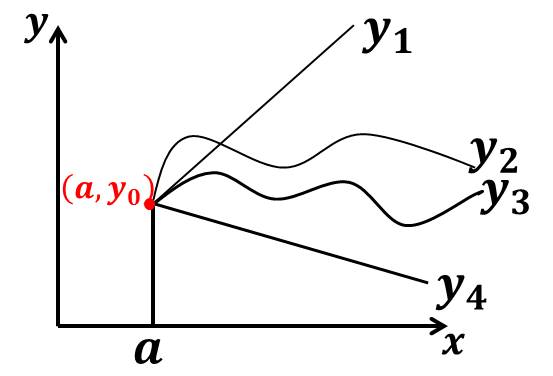
\includegraphics[width=4cm]{images/Initial_value_problems_of_ordinary_differential_equations.jpg}
		\caption{常微初值问题解的示意图}
		\label{fig:常微初值问题解的示意图}
		\end{figure}
		\noindent 注:$y$是$x$的函数,$y''$亦为$x$的函数。
		\par
		对于此问题,我们应该讨论问题解的存在性与唯一性(这个之前介绍过)。在解存在唯一的基础上,我们来考虑其数值解法。下面,我们介绍初值问题的欧拉法。
		\par
		我们先将$x$在$[a,b]$区间内离散化为$n$个点,这里为了方便,我们实现$n$等分。令$h=\frac{b-a}{n}$,有
		\[
			x_i=a+i\frac{b-a}{n}\quad i=0,1,\dots,n
		\]
		假设已知$x_i,y_i$,现在的问题是如何求$y_{i+1}$。
		\[
			y'(x_i)=f(x_i,y(x_i))
		\]
		而
		\[
			y'(x_i)=\frac{y(x_{i+1})-y(x_i)}{h}-\frac{h}{2}y''(\xi_i)
		\]
		故
		\[
			y_{i+1}\triangleq y(x_{i+1})=y(x_i)+hf(x_i,y_i)+\frac{h^2}{2}y''(\xi_i)
		\]
		\par
		由此,可以进一步思考推广:既然$y'(x)=f(x,y)$,那么,我们对等式两边进行相同的操作后,等式仍然成立。接下来,我们应该考虑的是:对于同一个问题,我们会有各种不同的解法,我们应该如何评价它们呢?对于此问题,这里不做讨论。
		\par
		常用的常微初值问题的数值解法是(4阶)Runge-Kutta方法,R-K方法是单步方法,即求$y_{i+1}$时只需要有$y_i$即可,其计算精度高,但计算量大,我们在后面的“嫦娥3号”最优控制的直接参数解法中,构建非线性方程时引入了R-K,所以这里不做介绍。

	\subsection{常微分方程边值问题}
		\par
		为简单,我们来看一个二阶常微分方程边值问题:求一个函数$y$,$y$在$x=a$处有已知信息,在$x=b$处亦有已知信息,信息可能是$y$在$a$处的一阶导、二阶导或者三阶导,并且要求$y$满足方程$y''=f(x,y,y')$,$a<x<b$。例如:
		\begin{align*}
			\left\{
				\begin{aligned}
					&y''=f(x,y,y')\\
					&y(a)=\alpha\\
					&y(b)=\beta\\
					&a<x<b
				\end{aligned}
			\right.
		\end{align*}
		\par
		下面,来介绍常微边值问题的数值解法 - 差分法。该方法用数值微分公式代替微分方程和边值条件中的导数,略去误差项,将常微离散为一个差分方程组,之后将方程组的解作为方程的近似解。
		\par
		在点$(x_i,y_i)$处有
		\[
			y''(x_i)=f(x_i,y_i,y_i(x_i))
		\]
		而数值微分公式为
		\[
			y''(x_i)=\frac{y(x_{i-1})-2y(x_i)+y(x_{i+1})}{h^2}-\frac{h^2}{12}y^{(4)}(\xi_i)
		\]
		将二者结合,略去高阶项$y^{(4)}(\xi_i)$,有
		\begin{align*}
		\frac{y(x_{i-1}) - 2y(x_i) + y(x_{i+1})}{h} = f(x_i,y_i,y_i') \quad i =1,2,\dots,n-1
		\end{align*}
		上式即为差分方程组。
		\par
		当$y$的边值信息已知时$(y(a)=\alpha,y(b)=\beta)$,则差分方程组为
		\begin{align*}
		\left\{
			\begin{aligned}
			&\frac{y(a) - 2y(x_1) + y(2)}{h} = f(x_1,y_1,y_1') \quad i =1\\
			&\frac{y(x_{i-1}) - 2y(x_i) + y(x_{i+1})}{h} = f(x_i,y_i,y_i') \quad i =2,3,\dots,n-1 \\
			&\frac{y(x_{n-2}) - 2y(x_{n-1}) + y(x_{b})}{h} = f(x_i,y_i,y_i') \quad i =n
			\end{aligned}
		\right.
		\end{align*}
		解上述方程组,得到$\left\{y_i\right\}_{i=1}^n$即为$y$的离散值。

	\subsection{MATLAB解常微分方程}
		\subsubsection{常用函数说明}
			1、MATLAB中提供ode23、ode45、ode113、ode15s、ode23s、ode23t、ode23tb函数用于求解常微分方程(组)初值问题。关于函数的说明,可以参考表(\ref{tab:MATLAB常微初值问题函数表})
			\begin{table}[H]
			\caption{MATLAB常微初值问题函数表}
			\label{tab:MATLAB常微初值问题函数表}
			\newcolumntype{Y}{>{\centering\arraybackslash}X}% 定义自适应列的居中格式 Y, 用 X 为左对齐(自适应列)
			\begin{tabularx}{\textwidth}{|c|c|c|X|}% 需要引入 tabularx 宏包;表格总宽度一定要设置
			\hline
			函数 & 问题类型 & 精确度 & 说明\\
			\hline
		ode45 & 非刚性 & 中等 & 采用算法为4-5阶Runge-Kutta法,是大多数情况下首选的函数\\\hline
		\multirow{2}*{ode23} & \multirow{2}*{非刚性} & \multirow{2}*{低} & 基于Bogacki-Shampine2-3阶Runge-Kutta公式,在精确度要求不高的场合,以及对于轻度刚性方程,ode23的效率可能好于ode45\\\hline
		\multirow{5}*{ode113} & \multirow{5}*{非刚性} & \multirow{5}*{低到高} & 基于变阶次Adams-Bashforth-Moutlon{}PECE算法。在对误差要求严格的场合或者输入参数odefun代表的函数本身计算量很大情况下比ode45效率高。ode113可以看成一个多步解算器,因为它会利用前几次时间点上的解计算当前时间节点的解。因此它不适应于非连续系统\\\hline
		\multirow{4}*{ode15s} & \multirow{4}*{刚性} & \multirow{4}*{低到中} & 基于数值差分公式(反向差分公式,BDFs也叫Gear方法),因此效率不是很高。同ode113一样,ode15s也是一个多步解算器,当ode45求解失败,或者非常慢,并且怀疑问题是刚性的,或者求解微分代数问题时可以考虑用ode15s\\\hline
		\multirow{3}*{ode23s} & \multirow{3}*{刚性} & \multirow{3}*{低} & 基于修正的二阶Rosenbrock公式。由于是单步解算器,当精度要求不高时,它的效率可能会高于ode15s。ode23s可以解决一些ode15s求解起来效率不太高的刚性问题\\\hline
		ode23t & 适度刚性 & 低 & ode23t可以用来求解微分代数方程\\\hline
		ode23tb & 刚性 & 低 & 当方程是刚性的,并且求解要求精度不高时可以使用\\\hline
			\end{tabularx}
			\end{table}
			说明:常微的刚性和非刚性,直观上讲,在短时间内常微解$y(x)$有巨大波动变化的,称为刚性问题(stiff)。对刚性问题,如果使用ode45的话,一般会花费很大代价。
			\par
			上述表(\ref{tab:MATLAB常微初值问题函数表})中函数命令的一般格式为
			\par
			[t,y] = ode$\sim$(odefun,tspan,y0,options)\\
			其中:odefun为方程函数句柄;tspan为方程的时间长度;y0为初始条件;options为参数设置。
			\par
			2、MARLAB中提供dde23和ddesd函数用于处理延迟常微分方程(DDE)。前者用来求解状态变量延迟数为常数的微分方程(组),后者用来求解延迟非常数的微分方程(组),而ddensd用于求解中性类型延迟微分方程。延迟微分方程在常微分方程的基础上添加时延,一般形式为
			\[
				y'(t)=f(t,y(t),y(t-\tau_1),y(t-\tau_2),\dots,y(t-\tau_n))
			\]
			其中:$\tau_1,\tau_2,\dots,\tau_n>0$是时延,$y(t-\tau_1),y(t-\tau_2),\dots,y(t-\tau_n)$是时延项。
			\par
			延迟微分方程中,$y$在$t$时刻的状态增量$y'(t)$不仅与此时的状态$y(t)$有关,而且还与之前的状态$y(t-\tau_1),y(t-\tau_2),\dots,y(t-\tau_n)$有关。如果你不是很熟悉DDE,可以继续阅读后面章节,在后面章节中你会慢慢体会到延迟的思想。
			\par
			dde23函数命令格式为
			\par
			sol = dde23(ddefun,lags,history,tspan,options)\\
			其中:ddefun为时滞方程函数句柄;lags为时间延迟向量,其中,$\tau_k$保存在lags($k$)中;history是描述$t\leq t_0$时状态变量值的函数,可以是句柄也可以是常数;tspan 是时间区间;options是参数设置结构体;sol为输出结构体,包括:sol.x,sol.y,sol.yp,solver等。
			\par
			ddesd函数命令格式为
			\par
			sol = ddesd(ddefun,delays,history,tspan,options)\\
			其中:上述这个函数可以处理的延迟微分方程的一般形式为:
			\[y'(t)=f(t,y(t),y(d(1)),y(d(2)),\dots, y(d(k)))\]ddefun为时滞方程函数句柄,例如:dydt=ddefun(t,y,z),t对应当前时刻$t$,y是一个$y(t)$ 的近似列向量,z的第j个列向量对应$y(d(j))$的估计;delays为函数句柄,返回$d(j)$列向量,$d(j)$可以依赖于$t$和$y(t)$。
			\par
			ddensd函数命令格式为
			\par
			sol = ddensd(ddefun,dely,delyp,history,tspan,options)\\
			其中:上述这个函数可以处理的延迟微分方程的一般形式为:
			\[y '(t) = f(t, y(t), y(dy_1),..., y(dy_p), y '(dyp_1),..., y '(dyp_q))\]
			$t$ is the independent variable representing time;$dy_i$ is any of p solution delays;$dyp_j$ is any of q derivative delays.
			\par
			3、MATLAB中提供了bvp4c,bvp5c函数用于求解常微分方程边值问题。bvp4c和bvp5c函数具有相同的命令格式
			\par
			sol = bvp4/5c(odefun,bcfun,solinit,options)
			\par
			solinit = bvpinit(x, yinit, params)\\
			其中:bcfun为边值函数句柄;solinit为结构体:solinit.x为取值范围,solinit.y为初始猜测值,solinit.params为参数的初始猜测;options为参数结构体;x为时刻点,即边值时刻x=[a,b],如果是多点边值,x=[a,c,b];yint为解的初始猜测值$y(a)$。

		\subsubsection{函数示例}
			% \textcolor[rgb]{1.00,0.00,0.00}{这部分在程序文件夹“ODE”当中。}
			\par
			这里,我们先给出Euler方法的程序。用Euler方法求解如下常微分问题
			\begin{align*}
			\left\{
			\begin{aligned}
			& x'= -3x+6t+5\\
			& x(0) = 3
			\end{aligned}
			\right.
			\end{align*}
			上述问题的解析解为$x = 2e^{-3t}+2t+1$。求解程序如下
			\begin{lstlisting}[language = Matlab]
			L=1; h=0.05; t=0:h:L;
			x_Euler = zeros(length(t),1); x_Euler(1)=3;
			x_pc = x_Euler; x_ode45=x_Euler;
			for n=1:length(t)-1
			    %欧拉法
			    x_Euler(n+1) = x_Euler(n)+h*(-3*x_Euler(n)+6*t(n)+5);
			    %预测-校正法
			    k1 = h*(-3*x_pc(n) + 6*t(n)+5);
			    k2 = h*(-3*(x_pc(n)+k1) + 6*(t(n)+h)+5);
			    x_pc(n+1) = x_pc(n)+(k1+k2)/2;
			end
			%ode45
			[t,x_ode45]=ode45(@(t,x)[-3*x+6*t+5],t,x_ode45(1));
			%解析解
			x_exact = 2*exp(-3*t)+2*t+1;
			%画图
			figure
			plot(t,x_Euler,'xk',t,x_pc,'ok',t,x_ode45,'+k',t,x_exact,'k','MarkerSize',8,'LineWidth',1)
			axis([0 1 2.3 3.15]), set(gca,'Fontsize',8), xlabel t, ylabel x
			legend('欧拉法','预测-校正法','ode45','解析解','location','North')
			\end{lstlisting}
			求解结果如图(\ref{fig:Euler-ode模拟结果})所示
			\begin{figure}[H]
	        \centering
	        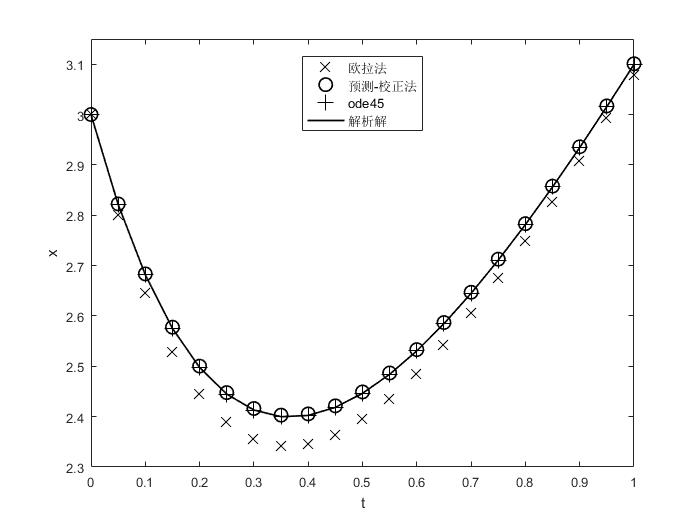
\includegraphics[width=8cm]{images/Euler-ode.jpg}
	        \caption{Euler方法求解常微分方程的结果}
	        \label{fig:Euler-ode模拟结果}
	        \end{figure}
	        \par
	        下面,我们给出一些MATLAB求解常微分的示例:(1)用ode45求解含参常微分方程初值问题
	        \begin{align*}
			\left\{
			\begin{aligned}
			& y''_1 - \mu \left( 1 - y_1^2\right) y'_1+y_1=0\\
			& y_1(0)=1,\ y_1(0)'=0\\
			& 0<t<30
			\end{aligned}
			\right.
	        \end{align*}
	        其中:$\mu > 0$是一个标量参数。设$y_1'=y_2$,重写上面的方程,有
	        \begin{align*}
			\left\{
			\begin{aligned}
			& y'_1 = y_2\\
			& y'_2 = \mu (1-y_1^2) y_2 - y_1\\
			& y_1(0)=1,\ y_1(0)'=0\\
			& 0<t<30
			\end{aligned}
			\right.
	        \end{align*}
	        求解程序为
	        \begin{lstlisting}[language = Matlab]
			tspan = [0, 30];
			y0 = [1, 0];
			odefun = @(mu)@(t, y)[y(2); mu*(1-y(1)^2)*y(2)-y(1)];
			mu = 2;
			[t,y] = ode45(odefun(mu), tspan, y0);
			plot(t, y(:,1),'-o', t, y(:,2),'-o')
			title('Solution of van der Pol Equation (\mu = 1) with ODE45');
			legend('y_1','y_2')
	        \end{lstlisting}
	        求解结果如图(\ref{ode45求解带参常微分方程})所示
			\begin{figure}[H]
	        \centering
	        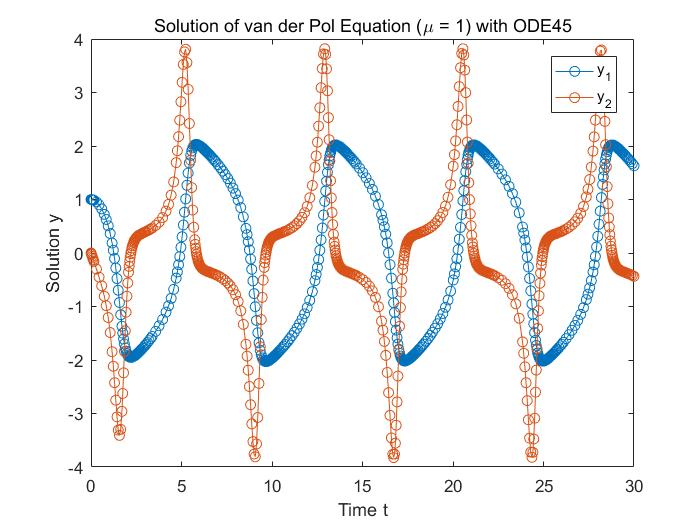
\includegraphics[width=8cm]{images/ode45solveParam.jpg}
	        \caption{ode45求解带参常微分方程}
	        \label{ode45求解带参常微分方程}
	        \end{figure}
	        (2)用ode15s求解刚性常微分初值问题。承继上面的问题,当$\mu=1000$时,在短时间内,函数值变化非常大,问题变为刚性问题,我们用ode15s求解如下刚性问题
	        \begin{align*}
			\left\{
			\begin{aligned}
			& y_1' = y_2\\
			& y_2' = 1000(1-y_1^2)y_2-y_1\\
			& y_1(0)=1,\ y_2(0)=0\\
			& 0<t<3000
			\end{aligned}
			\right.
	        \end{align*}
	        求解程序如下
	        \begin{lstlisting}[language = Matlab]
			mu = 1000;
			tspan = [0, 3000];
			y0 = [1, 0];
			[t,y] = ode15s(odefun(mu), tspan, y0);
			plot(t,y(:,1),'-o')
	        \end{lstlisting}
	        求解结果如图(\ref{ode15s刚性常微分初值问题})所示
			\begin{figure}[H]
	        \centering
	        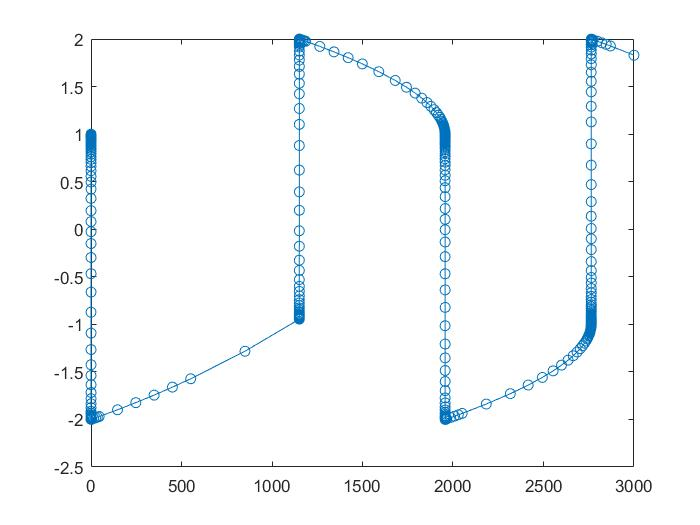
\includegraphics[width=8cm]{images/ode15sgangxing.jpg}
	        \caption{ode15s刚性常微分初值问题}
	        \label{ode15s刚性常微分初值问题}
	        \end{figure}
	        (3)用ode15i求解隐式常微分方程。上面展示的是显式常微分问题:$y'=(t,y)$ ,并且ode45和ode15s的微分方程函数句柄odefun要求方程为显式。下面,我们将展示隐式微分方程的求解,隐式常微分问题可以表示为
	        \begin{align*}
	        \left\{
	        \begin{aligned}
	        & f(t,y,y')=0\\
			& y(0)=y0\\
	        \end{aligned}
	        \right.
	        \end{align*}
	        对于隐式微分方程,我们一般用ode15i进行求解。作为示例,我们用ode15i求解Weissinger隐式问题:
	        \begin{align*}
	        ty^2(y')^3-y^3(y')^2+t(t^2+1)y'-t^2y=0
	        \end{align*}
	        求解程序如下
	        \begin{lstlisting}[language = Matlab]
			weissinger = @(t,y,yp)[t*y^2 * yp^3 - y^3 * yp^2 + t*(t^2 + 1)*yp - t^2 * y];
			t0 = 1;
			y0 = sqrt(3/2);
			yp0 = 0;
			[y0, yp0] = decic(weissinger, t0, y0, 1, yp0, 0);%为ode15i提供恰当的初始值
			tspan = [1, 10];
			[t,y] = ode15i(weissinger, tspan, y0, yp0);
			ytrue = sqrt(t.^2 + 0.5);
			plot(t,y,t,ytrue,'o')
	        \end{lstlisting}
	        求解结果如图(\ref{ode15i求解隐式常微分方程})所示
			\begin{figure}[H]
	        \centering
	        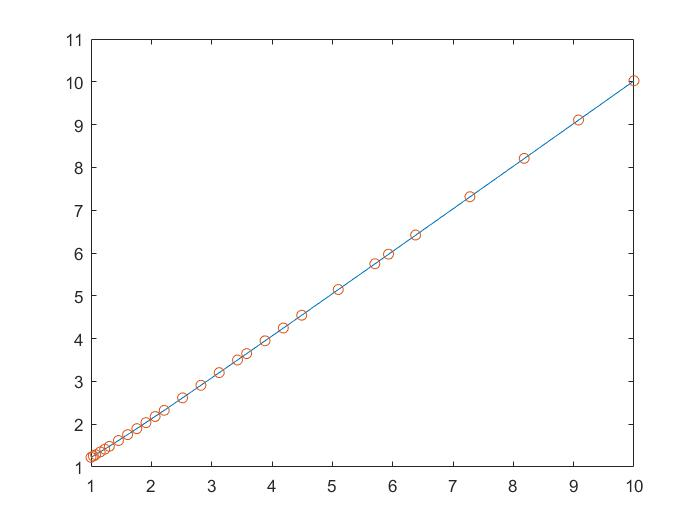
\includegraphics[width=8cm]{images/ode15iyinshifanghceng.jpg}
	        \caption{ode15i求解隐式常微分方程}
	        \label{ode15i求解隐式常微分方程}
	        \end{figure}
	        \par
	        (4)上面介绍了一些求解ODE初值问题的方法,下面我们来求解常微分方程边值问题。求解含参常微分方程边值问题,作为示例,我们求解Mathieu方程
	        \begin{align*}
			\left\{
			\begin{aligned}
			& y''+(\lambda-2q\cos2x)y=0\\
			& y'(0) = 0\\
			& y'(\pi)=0\\
			& y(0)=1
			\end{aligned}
			\right.
	        \end{align*}
	        其中: $\lambda$为参数。 求解第四特征值 $(q = 5)$ 的Mathieu方程,求解程序如下
	        \begin{lstlisting}[language = Matlab]
			lambda = 15;
			q = 5;
			mat4init = @(x)[cos(4*x); -4*sin(4*x)];%
			solinit = bvpinit(linspace(0,pi,10), mat4init, lambda);%求解迭代初始值。挑选一个满足y'(0)=0,y'(pi)=0,y(0)=1的函数(cos4x),-4sin(4x)为其导数
			mat4ode = @(q)@(x,y,lambda)[y(2);  -(lambda - 2*q*cos(2*x))*y(1) ];%微分方程匿名函数句柄
			mat4bc = @(ya,yb,lambda)[ya(2);yb(2); ya(1)-1 ];%边值条件
			sol = bvp4c(mat4ode(q),mat4bc,solinit);
			fprintf('The fourth eigenvalue is approximately %7.3f.\n',...
			        sol.parameters)
			xint = linspace(0,pi);
			Sxint = deval(sol,xint);
			figure, plot(xint,Sxint(1,:))
			axis([0 pi -1 1.1])
			title('Eigenfunction of Mathieu''s equation.')
	        \end{lstlisting}
	        求解结果如图(\ref{ode边值问题-求解Mathieu方程})所示
			\begin{figure}[H]
	        \centering
	        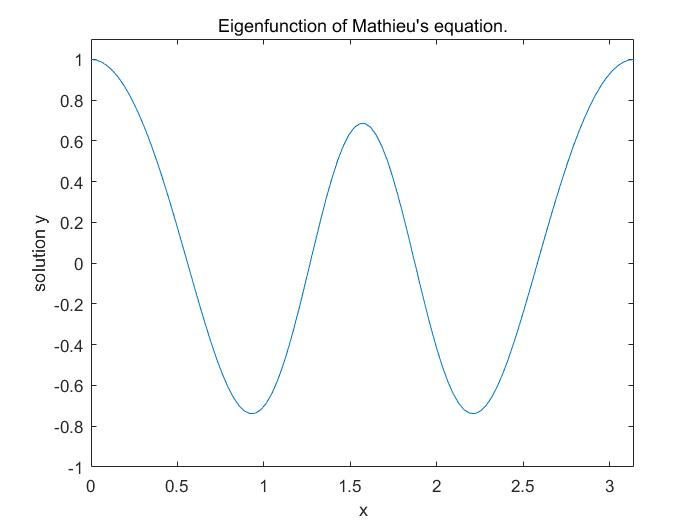
\includegraphics[width=8cm]{images/odebianzhiwenti.jpg}
	        \caption{Mathieu方程}
	        \label{ode边值问题-求解Mathieu方程}
	        \end{figure}
	        (5)求解延迟微分方程问题DDE。固定时滞的时滞微分方程描述为
	        \begin{align*}
	        y'(t)=f(t,y(t),y(t-\tau_1),...,y(t-\tau_k))
	        \end{align*}
	        其中:$\tau_i$为时滞长度,$y(t-\tau_i)$为时滞项。因为时滞长度为常数,所以被称为固定时滞微分方程。如果$\tau_i$不固定,而是与时间$t$ 或者$y$有关(表示为$d(t)$),则称为非固定延迟微分方程。求解下面的固定延迟微分方程:
	        \begin{align*}
			\left\{
			\begin{aligned}
			& y'_1(t) = y_1(t-1)\\
			& y'_2(t) = y_1(t-1)+y_2(t-0.2)\\
			& y'_3(t) = y_2(t)\\
			& 0<t<5
			\end{aligned}
			\right.
	        \end{align*}
	        小于初始时间的历史信息是:当$t \leqslant 0$时,$y_1(t) = 1,y_2(t) = 1,y_3(t) = 1$。将下面的程序保存为函数,以便后面的调用
	        \begin{lstlisting}[language = Matlab]
	         function dydt = ddex1de(t,y,Z)
		        % 延迟方程的函数
		        ylag1 = Z(:,1);%对所有延迟为delags(1)的状态变量的求解
		        ylag2 = Z(:,2);
		        %y1(t-1):状态变量为y1,延迟了delags(1),故用ylag1(1)表示。
		        dydt = [ ylag1(1)
		           ylag1(1) + ylag2(2)
		           y(2)               ];
		    end
	        \end{lstlisting}
	        求解程序为
	        \begin{lstlisting}[language = Matlab]
			tspan = [0, 5];
			delags = [1, 0.2];
			history = ones(3,1);
			sol = dde23(@ddex1de,delags,history, tspan);
			figure;
			plot(sol.x,sol.y)
			title('An example of Wille'' and Baker.');
			xlabel('time t');
			ylabel('solution y');
	        \end{lstlisting}
			求解结果如图(\ref{固定时滞的时滞微分方程})所示
			\begin{figure}[H]
	        \centering
	        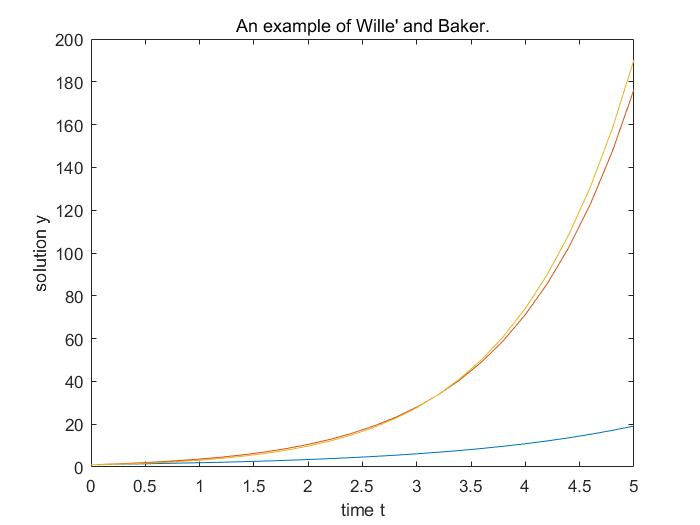
\includegraphics[width=8cm]{images/DDEgudingshizhi.jpg}
	        \caption{固定时滞的时滞微分方程}
	        \label{固定时滞的时滞微分方程}
	        \end{figure}
	        (6)求解下面非固定延迟微分方程,
	        \begin{align*}
			\left\{
			\begin{aligned}
			& y_1(t)'=y_2(t)\\
			& y_2'(t)=-y_2(\exp(1-y_2(t)))*y_2(t)^2*\exp(1-y_2(t))\\
			& 0.1<t<5
			\end{aligned}
			\right.
	        \end{align*}
	        其中:延迟函数$d(t) = \exp(1-y_2(t))$ 。该延迟微分方程有解析解 $y_1(t) = \log (t),y_2(t)=1/t$,可以作为时间小于初始时间$t<0.1$的历史信息。将下面的代码保存为函数,以便后面调用。
	        \begin{lstlisting}[language = Matlab]
			 function v = ddex3hist(t)
		    % 历史函数
		    v = [ log(t); 1./t];
		    end
		    function d = ddex3delay(t,y)
		    % 延迟函数
		    d = exp(1 - y(2));
		    end
		    function dydt = ddex3de(t,y,Z)
		    % 延迟方程
		    %由于只有一个延迟项,因此Z只有一列。
		    %y2(exp(1-y2(t)))延迟了exp(1-y2(t)),y2又是第二个状态变量,因此用Z(2)表示。
		    dydt = [ y(2); -Z(2)*y(2)^2*exp(1 - y(2))];
		    end
	        \end{lstlisting}
	        求解程序如下
	        \begin{lstlisting}[language = Matlab]
			t0 = 0.1;
			tfinal = 5;
			tspan = [t0, tfinal];
			sol = ddesd(@ddex3de,@ddex3delay,@ddex3hist,tspan);
			% Exact solution
			texact = linspace(t0,tfinal);
			yexact = ddex3hist(texact);
			figure
			plot(texact,yexact,sol.x,sol.y,'o')
			legend('y_1, exact','y_2, exact','y_1, ddesd','y_2, ddesd')
			title('D1 problem of Enright and Hayashi')
	        \end{lstlisting}
	        求解结果如图(\ref{非固定时滞的时滞微分方程})所示
			\begin{figure}[H]
	        \centering
	        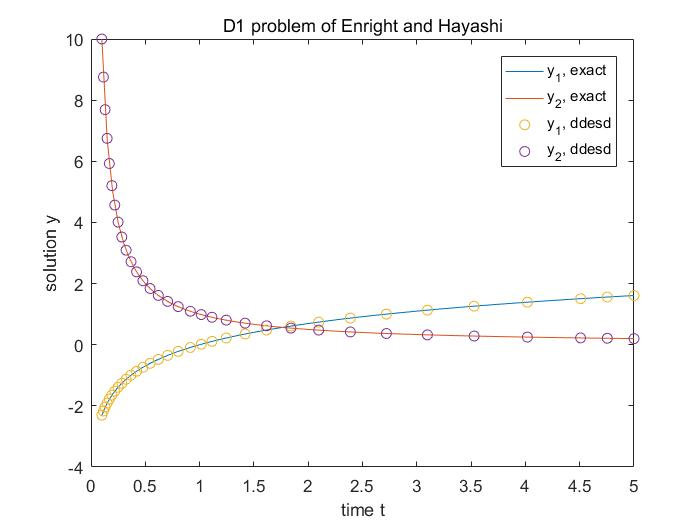
\includegraphics[width=8cm]{images/DDEfeigudingyanchi.jpg}
	        \caption{非固定时滞的时滞微分方程}
	        \label{非固定时滞的时滞微分方程}
	        \end{figure}
	        (7)求解下面的中性时滞微分方程:
	        \begin{align*}
			\left\{
			\begin{aligned}
			& y'(t)=1+y(t)-2y(t/2)^2-y'(t-\pi)\\
			& 0\leq t \leq \pi
			\end{aligned}
			\right.
	        \end{align*}
	        其中:$y(t)$的历史信息是:$t \leqslant 0$ 时,$y(t) = \cos (t)$。将下面的程序保存为函数,以便后面调用。
	        \begin{lstlisting}[language = Matlab]
		 	function yp = ddefun(t,y,ydel,ypdel)
		        yp = 1 + y - 2*ydel^2 - ypdel;
		    end
		    function dy = dely(t,y)
		        dy = t/2;
		    end
		    function dyp = delyp(t,y)
		        dyp = t-pi;
		    end
		    function y = history(t)
		        y = cos(t);
		    end
	        \end{lstlisting}
	        求解程序如下
	        \begin{lstlisting}[language = Matlab]
			tspan = [0 pi];
			sol = ddensd(@ddefun,@dely,@delyp,@history,tspan);
			tn = linspace(0,pi);
			yn = deval(sol,tn);
			plot(tn,yn);
			xlim([0 pi]);
			ylim([-1.2 1.2]);
	        \end{lstlisting}
	        求解结果如图(\ref{中性时滞微分方程})所示
			\begin{figure}[H]
	        \centering
	        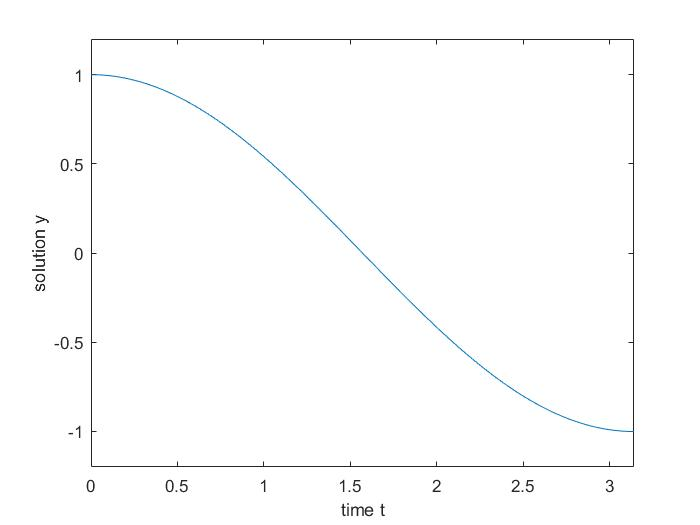
\includegraphics[width=8cm]{images/zhongxingDDE.jpg}
	        \caption{中性时滞微分方程}
	        \label{中性时滞微分方程}
	        \end{figure}

\section{常微分方程稳定性}
	\par
	微分方程(组)的解析法(初等方法)经历了很漫长的研究。19世纪中下,刘维尔的工作表明:绝大多数微分方程(组)不能用初等方法进行求解。前面,我们谈到微分方程(组)的解存在唯一性及其解析方法。但刘表明,绝大多数微分方程求不出解析解。为此,我们有必要研究一下解$(x(t))$的其它性质。法国数学家庞加莱(1852-1912)发展了解的定性理论,俄罗斯数学家李雅普诺夫(1857-1918)创立了解的稳定性理论。二者的共同特点是在不求解方程(组)的情况下,直接依据方程本身的结构特点来研究定解的性质。
	\par
	下面,我们来介绍微分方程组的稳定性。考虑下面的微分方程组
	\[
		\dot{\mathrm{x}}=F(t,\mathrm{x})
	\]
	其中:$F$对$\mathrm{x}\in D\subset R^n$和$t\in R$连续,并且对$\mathrm{x}$满足利普西茨条件,即解存在唯一。
    \par
    系统(方程组)中可以有一个变量或者多个变量。稳定性问题的实质是考察系统$\mathrm{x}(t)$(为简便,将$\mathrm{x}(t)$记为$x(t)$)由初始状态$x_0$扰动$x_0+\Delta x$引起的受扰运动$x(t;t_0,x_0)$能否趋近于或者返回平衡状态。
    \par
    平衡状态是指:不受外界干扰的情况下,系统状态$x(t)$不随时间$t$变化而变化;稳定状态是指:系统状态$x(t)$不随时间$t$变化而变化。由于我们并不考虑外界干扰,故平衡态为$\dot{x}(t)=\frac{\mathrm{d}x}{\mathrm{d}t}=0$。若已知$F(x,t)$的函数形式,我们可以用$F(x,t)=0$来求平衡态,不妨设平衡态为$x_e$。
    \par
    再用数学语言描述一下稳定性:设方程对初值$(t_0,x_0)$存在唯一解$x_0(t;t_0,x_0)$,而对其它初值$(t_0,x_1)$存在唯一解$x_1(t;t_0,x_1)$。稳定性是指:当$||x_1-x_0||$很小的时候,$||x_1(t;t_0,x_1)-x_0(t;t_0,x_0)||$是否也很小。如果从系统运动图像来看,可以表现为$x(t)$对初值的敏感性问题:如系统稳定性示意图如图(\ref{fig:系统稳定性示意图})所示
	    \begin{figure}[H]
	    \centering
	    \begin{varwidth}[t]{\textwidth}
	    \vspace{0pt}
	    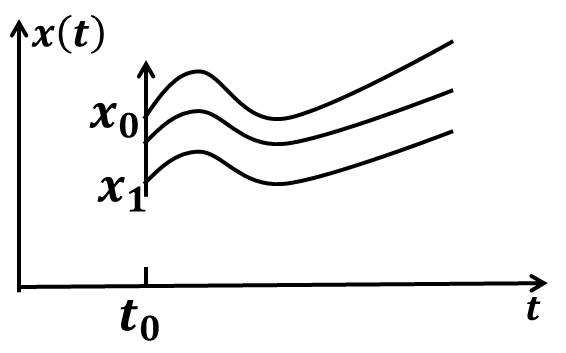
\includegraphics[width=4cm]{images/xtwdxsyt1.jpg}
		\end{varwidth}
		\qquad \qquad
		\begin{varwidth}[t]{\textwidth}
		\vspace{0pt}
		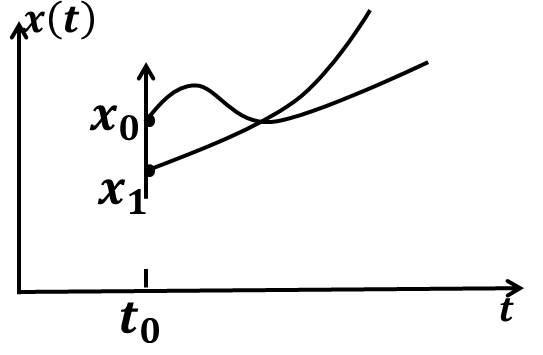
\includegraphics[width=4cm]{images/xtwdxsyt2.jpg}
		\end{varwidth}
		\caption{系统稳定性示意图}
		\label{fig:系统稳定性示意图}
		\end{figure}
    % \textcolor[rgb]{1.00,0.00,0.00}{todo:图片:系统稳定性示意图}\\
    \subsection{李雅普诺夫意义下的稳定}
        \par
        1.李雅普稳定是指:初始条件$x_0$在平衡状态$x_e$附近的任意一个初始状态的运动轨迹$x(t;t_0,x_0)$均维持在平衡状态$x_e$的附近。
        \par
        设系统的初始状态为$(t_0,x_0)$,平衡态$x_e$,初始状态的运动轨迹为$x(t;t_0,x_0)$。如果对于每个实数$\varepsilon>0$,都存在另一个实数$\delta (\varepsilon , t_0)>0$ ,$x_0$位于以$x_e$为球心,$\delta$为半径的闭球域$S(\delta)$内,即$x_0\in S(\delta)$,或者写为
        \[
            ||x_0-x_e||\leq \delta (\varepsilon,t_0)\quad t=t_0
        \]
        由球域内的任意初始状态$x_0$出发的运动轨迹$x(t;t_0,x_0)$,在$t\rightarrow\infty$时,都位于以$x_e$为球心,以$\forall \varepsilon >0$为半径的球域$S(\varepsilon)$内,即
        \[
            ||x(t;x_0,t_0)-x_e||\leq\varepsilon\quad t\geq t_0
        \]
        则$x_e$为李雅普稳定,如图(\ref{fig:李雅普稳定示意图})所示,轨迹$x(t)$围绕$x_e$波动且不会逃出$S(\varepsilon)$。
         \begin{figure}[H]
        \centering
        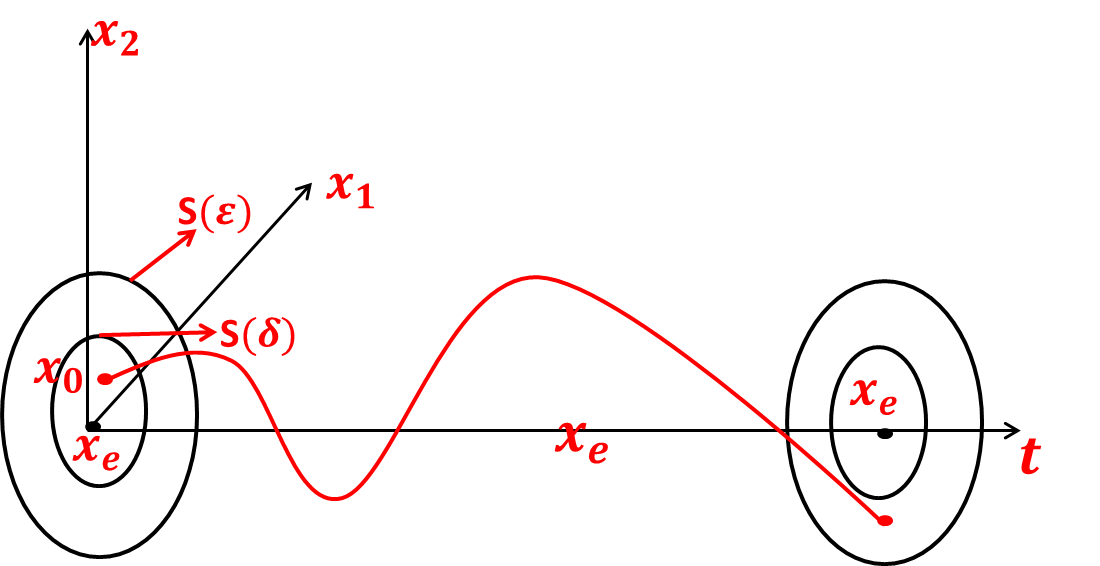
\includegraphics[width=8cm]{images/lypwdsyt.jpg}
        \caption{李雅普稳定示意图}
        \label{fig:李雅普稳定示意图}
        \end{figure}
        \par
        2.李雅普渐进稳定是指:从域$S(\delta)$出发的轨迹$x(t)$不仅不会超出$S(\varepsilon)$,而且当$t\rightarrow\infty$时,$x(t)$收敛于$x_e$。即李雅普渐进稳定首先要求是李雅普稳定,然后,$t\rightarrow\infty$时,有
        \[
            \lim_{t\rightarrow\infty}||x(t;x_0,t_0)-x_e||\rightarrow 0
        \]
        \par
        若$\delta$与$t_0$无关,且上式的极限过程与$t_0$无关,则称平衡状态$x_e$是一致渐进稳定,如图(\ref{fig:李雅普渐进稳定示意图})所示
         \begin{figure}[H]
        \centering
        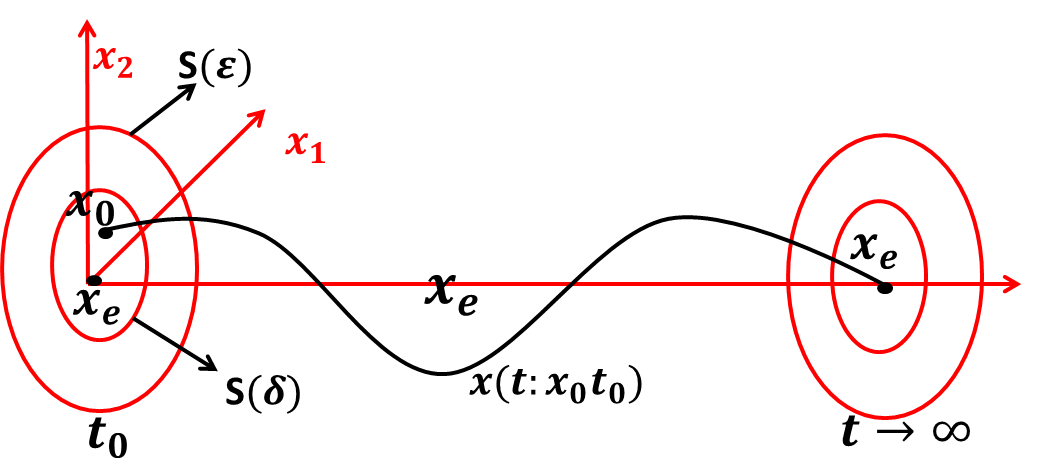
\includegraphics[width=8cm]{images/lypjjwdsyt.jpg}
        \caption{李雅普渐进稳定示意图}
        \label{fig:李雅普渐进稳定示意图}
        \end{figure}
        \par
        3.李雅普大规模渐进稳定是指:将李雅普渐进稳定的初始条件扩展到整个状态空间时的渐进稳定,换句话说,就是无论什么样的初始条件,都会稳定。对$\forall x_0\in S(\delta),\delta\rightarrow\infty ,S(\delta)\rightarrow\infty$,都有
        \begin{align*}
        \lim_{t\rightarrow\infty}||x(t;x_0,t_0)-x_e||\rightarrow 0
        \end{align*}
        \par
        4.李雅普不稳定是指:如果对某个实数$\varepsilon>0$,和任意实数$\delta >0$,不管$\varepsilon, \delta$有多小,在$S(\delta)$内,都存在一个初始状态$x_0$,$x_0$出发的轨迹都超出$S(\varepsilon)$,则平衡状态$x_e$称为李雅普不稳定。
    \subsection{李雅普第二方法(直接法)}
        上面,我们介绍了稳定性的概念,但是根据定义来判别$x_e$的稳定性是非常局限的,下面,我们介绍用李雅普第二方法来判断系统的稳定性。
        \paragraph{李雅普函数$V$}虚构一个能量函数$V$,$V$一般与$x,t$有关,记为$V(x,t)$,注意:$x$是$t$的函数$x(t)$。为了简单,不妨假设$V$不是时变的,即$V$不显含$t$,记为$V(x):=V(x(t))$。
        \par
        $V(x)$为$n$维矢量$x$定义的标量函数,$x\in \varOmega$,且在$x=0$时,$V(x)=0$。我们先来定义能量函数$V$的正定性:
        \par
        1、如果$V(x)>0$,则$V$为正定。例如:$V(x)=x_1^2+2x_2^2$,这里,系统共有两个变量$x_1,x_2$;
        \par
        2、如果$V(x)\geq0$,则$V$为半正定;
        \par
        3、如果$V(x)<0$,则$V$为负定;
        \par
        4、如果$V(x)\leq 0$,则$V$为半负定;
        \par
        5、如果$V(x)> 0$或者$V(x)< 0$,则$V$为不定;
        \par
        上面,我们简单介绍了李雅普函数,下面,就用李雅普函数$V(x)$来判定系统的稳定性。设系统状态方程为
        \[
            \dot{x}=F(x,t)
        \]
        系统的平衡状态为$F(x,t)=0$,即$x_e$。我们有如下李雅普稳定判定方法:
        \par
        1.若$\dot{V}=\frac{\mathrm{d}V}{\mathrm{d}t}\geq0$,则$x_e$为李雅普稳定。
        \par
        2.若$\dot{V}=\frac{\mathrm{d}V}{\mathrm{d}t}<0$,或者写为$\dot{V}\leq0$和$\forall x\in \varOmega$,$\dot{V}(x(t;x_0,t_0))$不恒等于0,则$x_e$为李雅普渐进稳定。
        \par
        3.若$\dot{V}<0$,并且,当$||x||\rightarrow\infty$时,$V(x)\rightarrow\infty$,则$x_e$为李雅普大范围渐进稳定。
        \par
        4.若$\dot{V}>0$,则$x_e$为李雅普不稳定。
        \par
        上述判据是判定系统是否稳定的充分条件。接下来我们应该思考的是:如何选取(构造)函数$V(x)$?其实,$V(x)$的选取并不唯一,并且很主观,很方便,没有统一的选取方法。在非线性系统下,可以依据雅可比矩阵法和变量梯度法进行选取。

\section{混沌理论Chaos}
    \subsection{混沌系统的引入}
        \par
        在介绍混沌理论之前,我们先来看两个例子:logistic映射和Lorenz方程。(1)logistic映射为
        \[
            x_{t+1}=\lambda x_t (1-x_t)
        \]
        毫无疑问,这是一个含参$\lambda$的一维动力系统(离散常微分方程),在给定初值条件$t_0=1$,$x(1)=x_0$时,会有它的运动轨迹$x_t$。下面,我们来研究一下运动轨迹的几种情况,如图(\ref{logistic映射对参数和初值的敏感性})所示
	    \begin{figure}[H]
	        \centering
	        \begin{subfigure}[b]{0.4\textwidth}
	            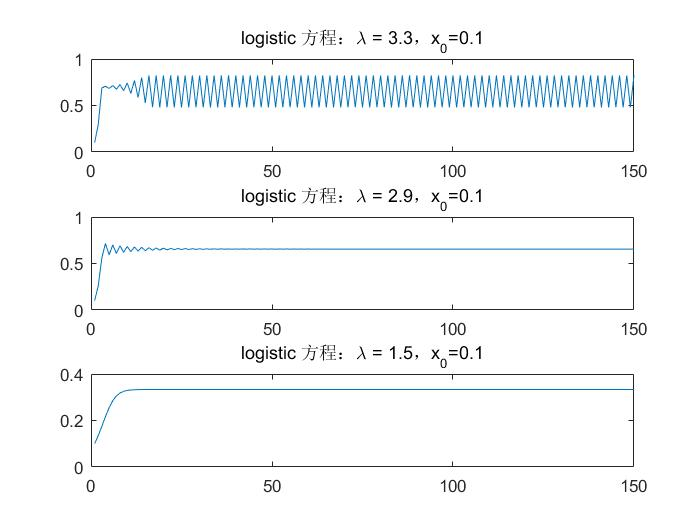
\includegraphics[width=\textwidth]{images/logistic-lambda.jpg}
	            \caption{logistic映射对初值的敏感性}
	            \label{logistic映射对初值的敏感性}
	        \end{subfigure}
	        \begin{subfigure}[b]{0.4\textwidth}
	            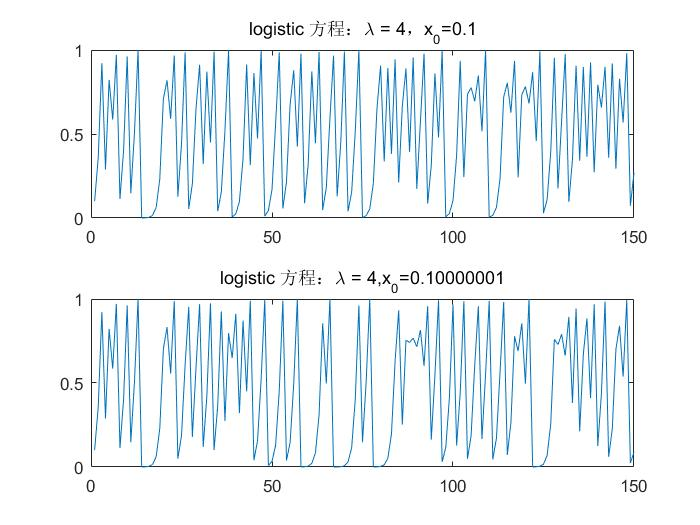
\includegraphics[width=\textwidth]{images/logistic-x0.jpg}
	            \caption{logistic映射对参数的敏感性}
	            \label{logistic映射对参数的敏感性}
	        \end{subfigure}
	        \caption{logistic映射对参数和初值的敏感性}
	        \label{logistic映射对参数和初值的敏感性}
	    \end{figure}
        \par
        上面的前3张图(\ref{logistic映射对初值的敏感性})是为了说明logistic映射对参数$\lambda$的敏感性,后两张图(\ref{logistic映射对参数的敏感性})是为了说明logistic映射对初始条件$x_0$的敏感性。由上面这个例子我们可以看出,虽然已经确定了运动方程$\dot{x}=f(x,t)$,但是其运动轨迹(方程的解)$x_t$却对初始条件及参数极为敏感,其轨迹曲线表现出不可预测,类似于随机性运动。虽然依据$\dot{x}=f(x,t)$以及$x(t_0)=x_0$,我们能够推算出来未来任意时刻$t$的运动状态$x_t$,但初始数据测量的不准确导致了整体测量的误差极大,甚至不可预测。20世纪70年代后的研究表明:大量非线性系统尽管状态方程是确定的,却普遍存在初值敏感问题,运动状态类似于随机运动。下面的工作就是简单研究一下这个初值敏感的确定系统(混沌系统)。
        \par
        (2)在介绍混沌(chaos)之前,我们再来看一个著名的初值敏感的例子 - Lorenz方程。美国气象学家Lorenz在研究大气对流时,建立了Lorenz方程,下面用一个简单的模拟模型来导出Larenz方程。
         \begin{figure}[H]
        \centering
        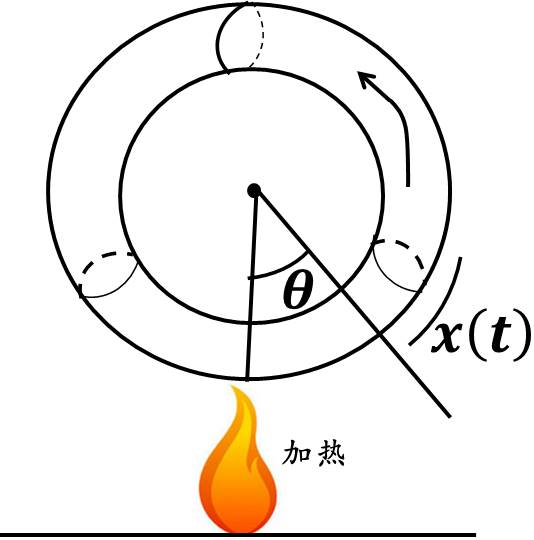
\includegraphics[width=3cm]{images/Atmospher_convection_simulation.jpg}
        \caption{大气对流模拟示意图}
        \label{fig:大气对流模拟示意图}
        \end{figure}
        \par
        模拟模型的示意图如图(\ref{fig:大气对流模拟示意图})。一个环形管内装满水,从下方点火加热,管内的水发生对流,设水是不可压缩的,对流时各处的瞬时速度是一样的,速度为$x(\theta ,t)$。由于不可以压缩,我们有$x$与$\theta $无关,即写为$x(t)$,令管的半径为1,管的截面积为1单位,$\nu $为粘度,$- \nu x$为流动阻力,再设管子上的温度为$T$,温度按高度线分布,即
        \[
            T_1=T_0+\Delta T \cos \theta
        \]
        其中:$T_0$与$\Delta T$为常数。
        \par
        管内流体的温度$T$为
        \[
            T = T_1+y(t)\sin \theta -z(t)\cos \theta
        \]
        其中:$z(t)$为管与液体间温度差的对称部分,$y(t)$为温差左右不对称部分,图(\ref{fig:大气对流模拟示意图})中左半部分液体较凉,右半部份液体较热,于是有
        \[
            \frac{\mathrm{d}x}{\mathrm{d}t} = - \nu x + k y
        \]
        \par
        考虑一段管子$\mathrm{d}\theta $的热平衡,流入与流出的液体的温差为$\frac{\partial T}{\partial \theta }\mathrm{d}\theta$,带走的热量为$\kappa x\frac{\partial T}{\partial \theta }\mathrm{d} \theta$,管壁传给流体的热量为$(T_1-T)\mathrm{d}\theta $,流体随时间吸收的热量为$\frac{\partial T}{\partial t}\mathrm{d}\theta$。于是,由热能守恒有
        \[
            \frac{\partial T}{\partial t} = -x\frac{\partial T}{\partial \theta } + \kappa (T_1-T)
        \]
        即
        \[
            \dot{y}(t)\sin \theta -\dot{z}(t) \cos \theta = -x [-\Delta T \sin \theta + y\cos \theta +z\sin \theta ] + \kappa(-y\sin \theta+z\cos \theta)
        \]
        令$\sin \theta\cos \theta$前的系数左右相等,有
        \begin{align*}
        &\dot{y} = \Delta T x - xz - \kappa y \\
        &\dot{z} = xy - \kappa z
        \end{align*}
        不妨令
        \[
            x = \kappa x,y=\frac{\nu \kappa}{k}y, z=\frac{\nu \kappa}{k}z
        \]
        再令
        \[
            t = \frac{1}{\kappa},\rho = \frac{\Delta T k}{\kappa \nu },\sigma = \frac{\nu }{\kappa}
        \]
        由此,可以得到Lorenz方程
        \begin{align*}
        	\left\{
        		\begin{aligned}
        		&\dot{x} = \sigma(y-x)\\
		        &\dot{y} = x(\rho -z) - y\\
		        &\dot{z} = xy - \beta z
        		\end{aligned}
        	\right.
        \end{align*}
        \par
        我们设置参数值为$\sigma = 10$,$\rho = 28$,$\beta = \frac{8}{3}$,$x_0=12$,$y_0=2$,$z_0=9$计算得到它们在三维空间上的曲线,以及$xy,yz,xz$面的投影和$x,y,z$变量各自的运动轨迹,如下面图(\ref{Lorenz仿真图})所示
	    \begin{figure}[H]
	        \centering
	        \begin{subfigure}[b]{0.4\textwidth}
	            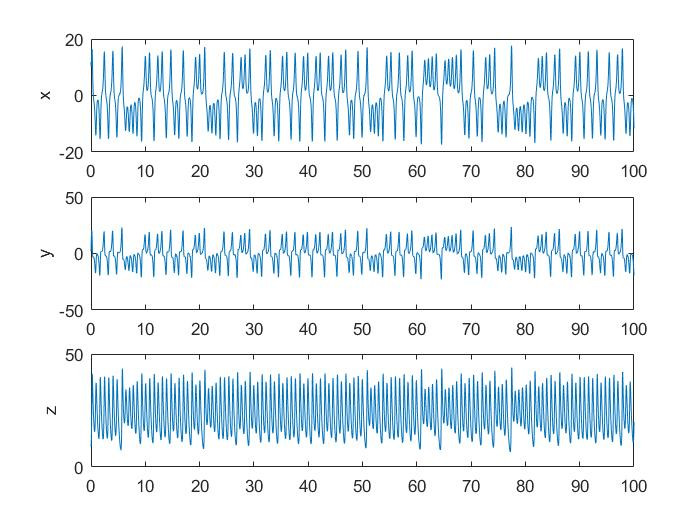
\includegraphics[width=\textwidth]{images/Lorenzguijixian.jpg}
	            \caption{Lorenz 一维轨迹线}
	            \label{Lorenz 一维轨迹线}
	        \end{subfigure}
	        \begin{subfigure}[b]{0.4\textwidth}
	            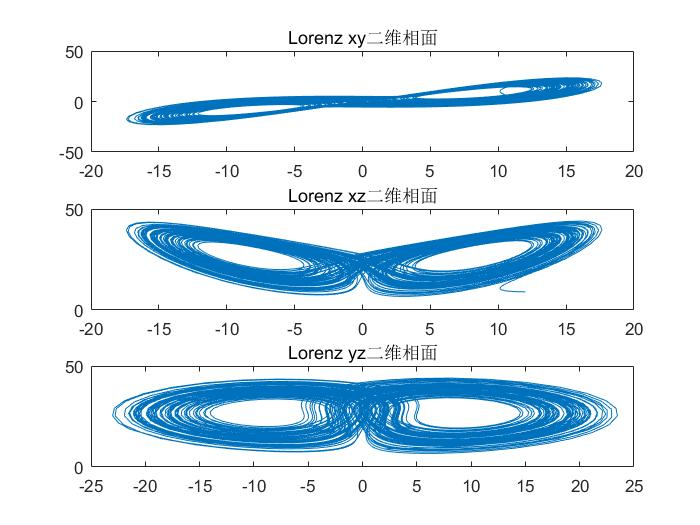
\includegraphics[width=\textwidth]{images/Lorenz2xiangmian.jpg}
	            \caption{Lorenz 二维相面}
	            \label{Lorenz 二维相面}
	        \end{subfigure}
	        \begin{subfigure}[b]{0.4\textwidth}
	            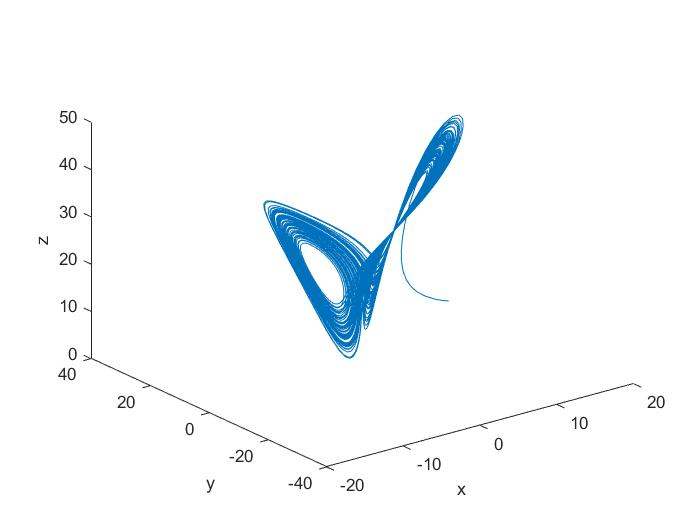
\includegraphics[width=\textwidth]{images/Lorenzxiangkongjian.jpg}
	            \caption{Lorenz 三维相空间}
	            \label{Lorenz 三维相空间}
	        \end{subfigure}
	        \caption{Lorenz仿真图}
	        \label{Lorenz仿真图}
	    \end{figure}
	    \par
        改变系统的初始值,会得到另一个完全不一样的结果:洛伦兹方程的解对初始值十分敏感,现对$y$的初始值稍加修改,将2改为2.01和1.99,让后求解$z$的数值解,如图(\ref{Lorenz初值敏感性实验})所示,随着时间的推移,三条曲线的吻合程度越来越差,差距越来越大,变化也越来越不明显,成为混沌状态。
        \begin{figure}[H]
        \centering
        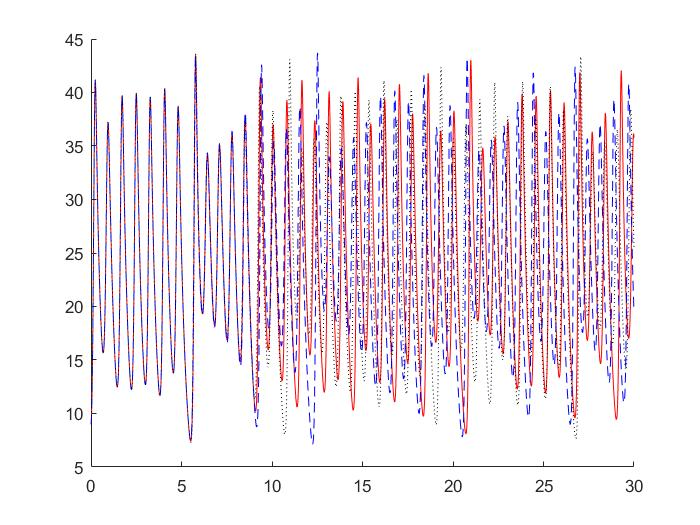
\includegraphics[width = 6cm]{images/Lorenzeffect.jpg}
        \caption{Lorenz初值敏感性实验}
        \label{Lorenz初值敏感性实验}
        \end{figure}
        注:上面轨迹中的不完全自我重复,轨迹不相交缺永不停止转动的双螺旋线即为“Lorenz吸引子”,在Lorenz方程之后,法国天文学家Henon提出了Henon映射方程。

    \subsection{混沌的基本理论}
        \paragraph{混沌现象}混沌是指确定的动力系统因为初值敏感而表现出的不可测的,类似随机的运动。哈密顿原理将动力学系统划分为可积与不可积两部分,可积系统的典型行为是周期运动和准周期运动,而混沌是不可积系统的典型行为。俄国数学家Lyapunov发明了运动系统的稳定性,同时,还提出了描述混沌运动的重要指标量 - Lyapunov指数,该指数是系统稳定性的关键。庞加莱在研究三体问题时发现了混沌,并用拓扑学的方法来解决问题。现代动力学系统理论的稳定性理论、分岔理论、奇点理论和吸引子等皆源于庞的研究。19世纪末,庞在研究三体运动时,发现了三体系统的不可积和轨道的复杂性,直到20世纪60年代初,三位数学家A.柯尔莫格洛夫、V.阿诺尔德和J.莫赛证明了KAM定理后,才从一定意义上回答了这个问题。
        \par
        20世纪50-60年代为混沌理论发展的初期(Lorenz系统),20世纪70年代是快速发展时期,混沌和吸引子等概念被提出,20世纪80年代混沌系统的定量研究成为热点。1980年,数学家Mandelbrot给出了第一张混沌图像,Mandelbrot集被公认为是混沌的一种标志。混沌系统的性质量:分数维、lyapunov指数、Kolmorov熵等的出现使混沌理论进入应用阶段。
        \paragraph{混沌的定义}混沌至今还没有一个统一的定义。下面,我们给出两个影响广泛的定义:Li-Yorke和Devaney的混沌定义。
        \par
        1975年,马里兰大学数学家Yorke和他的学生Li(李天岩)在论文《Period three means chaos》中给出了混沌的第一个数学定义:
        \begin{definition}[Li 混沌]
        设$f$是$[a,b]$上的连续自映射,其点映射形式为$x_{t+1}=f(x_t,\lambda)$,$x_n\in [a,b]$,$f$为混沌映射(混沌方程),如果\\
        (1)$f$的周期点的周期无上界,即$f$存在一切周期的周期点。\\
        (2)存在不可数的子集$s\subset[a,b]$,$s$中无周期点,且满足\\
        \ding{172}$\forall x,y\in s,x\neq y$,有
        \[
            \lim_{n\rightarrow\infty}\inf|f^n(x)-f^n(y)|=0
        \]
        \ding{173}$\forall x,y\in s,x\neq y$,有
        \[
            \lim_{n\rightarrow\infty}\sup|f^n(x)-f^n(y)|>0
        \]
        \ding{174}$\forall x \in s$,$f$的任意周期点$p$,有
        \[
            \lim_{n\rightarrow\infty}\sup|f^n(x)-f^n(p)|>0
        \]
        其中:$f^n(x)=f(f^n-1(x))=f(f(\dots f(x)))$。
        \end{definition}
        \par
        Li-Yorke的混沌定义中的\ding{172}和\ding{173}表明子集$s$中的点$x,y$相当分散又相当几种,\ding{174}表明子集$s$不会趋于任意周期点。
        \begin{theorem}[Li-Yorke定理]
        设$f$在$[a,b]$上连续自映射,若$f$有3这个周期点,则对于任意正整数$n$,$f$有$n$周期点。
        \end{theorem}
        \par
        由Li-Yorke定理和Li-Yorke混沌的定义,我们可以看到:如果$f$周期点3,那么$f$有任意整数周期点,故$f$混沌。
        \par
        另一个著名的混沌定义是Devaney的混沌定义:
        \begin{definition}[Devaney 混沌]
        设$D$是紧度量空间($[a,b]$),$f$为$D\rightarrow D$的连续映射,并且满足:\\
        \ding{172}$f$对初值敏感依赖,即$\exists \delta > 0,\forall \varepsilon > 0,\forall x \in D$,在$x$的$\varepsilon$邻域内,$\exists y,n$使得
        \[
            d[f^n(x),f^n(y)]>\delta
        \]
        \ding{173}$f$有拓扑传递性,对$D$上任意开集$X,Y$,$\exists k>0$,$f^k(X)\cap Y \neq \phi$。\\
        \ding{174}的周期点在$D$内稠密。\\
        则$f$为Devaney意义下的混沌。
        \end{definition}
        \par
        条件\ding{172}意味着无论初值依赖多近,在$f$的多次作用之后,二者之间的距离$d$都会超出$\delta$。条件\ding{173}意味着任意点的邻域在$f$的多次作用下将遍及整个度量空间$D$,这说明$f$不可能分解为两个在$f$下互不影响的子系统。条件\ding{174}意味着混沌系统存在着规律性成分。
        \par
        上面,我们给出了混沌的定义,在给出定义之后,接下来我们应该考虑的内容是:
        \begin{enumerate}
       \item 如何判定一个系统是混沌的?
        \item 混沌系统有哪些特征(性质)?
        \item 我们可以用混沌系统来做什么?
        \end{enumerate}
        \par
        对于1和2,其实二者之间是具有联系的,因为我们可以根据混沌系统的特性来判断一个系统是否是混沌系统。为此,我们有必要先来了解一下混沌系统的性质。
    \subsection{混沌的基本性质}
        \paragraph{吸引子}观察Lorenz系统的状态轨线图(\ref{Lorenz仿真图}),会发现状态的轨线好像被什么吸住了,但又在两个“蝴蝶翅膀”上蹦来蹦去。没错,能“吸住”轨线的那个东西(set)就是所谓的吸引子了,它使得一切运动趋向吸引子,而一旦到达吸引子内,运动就开始互相排斥。一般来讲,把$t\rightarrow\infty$时状态的“归宿”称为吸引子(吸引子是空间中的一个点,或者一个点集)。通常,吸引子被分为两类:1、平凡吸引子;2、奇异吸引子。而平凡吸引子又分为:1.不动点吸引子(平衡运动);2.极限环(周期运动);3.整数维环面(准周期运动)。吸引子是相空间中的一个集合(set)。下面给出吸引子的数学定义:
        \par
        设$A$是映射$f$的不变集,即$\lim_{t\rightarrow\infty}f^t(A)$,$f(A)=A$,其中:$f^t$表示$f$作用$t$次。若对$A$的每个$\varepsilon$邻域$S(\varepsilon)=\{x|d(x,A)<\varepsilon\}$,存在$A$的一个$\delta$邻域$S(\delta)$,使得$\forall p \in S_\delta $,有$f^t(p)\in S_\varepsilon$,$t\in \mathbb{N}$,则$A$为稳定集。
        \par
        若$A$为稳定集,又$\exists a > 0$,$\forall Q \in S_\delta $,在$t\rightarrow\infty$时,$d(f^t(Q),A)\rightarrow 0$,则$A$为渐进稳定集。若$A$为闭的渐进稳定不变集,则$A$为吸引集;吸引集中含稠密轨线时,即$\exists s \in A$,使得$\left\{f^t(s),t=1,2,\dots \right\}$的闭包等于$A$,则$A$称为吸引子。\\
        注:1.吸引子是一个集合。
        \par
        2.\ 2维时,相空间即为相平面。
        \par
        3.\ 吸引子是(相)空间中的一个集合。
        \par
        4.\ 相空间一般来说就是状态空间$\Omega=\{x(t)\}$。
        \paragraph{相空间 Phase Space}因为后面要讨论相空间重构的问题,所以这里简单介绍一下相空间。相:系统的具体某一状态$x(t)$。相空间即为状态空间,运动系统所有可能的状态取值的集合$\Omega=\{x(t)\}$。
        \par
        我们为什么要讨论吸引子?吸引子其实就代表了系统,如果系统具有奇异吸引子,那么这个系统就是混沌的。研究发现,奇异吸引子具有分数维(与整数维相对)、正的Lyapunov指数和正的Kolmogrov熵等特性,这些性质是平凡吸引子不具备的。由此,我们可以通过计算吸引子的特征量(分数维、Lyapunov指数和Kolmogrov熵等)来判断一个系统是否有奇异吸引子,从而判断一个系统是否是混沌系统。下面,我们来介绍吸引子的3种特征量,以及它们在相空间重构基础上的数值解法。

        \paragraph{吸引子的2个特征量}1.描述邻近轨道发散率的Lyapunov指数或者最大Lyapunov指数谱。
        我们考虑一个一维映射$x(t+1)=f(x(t))$,假设初始条件$x(t_0)$附近有一点$x(t_0)+\delta x(t_0)$,则经过$n$次迭代后,有
        \[
            \delta x(t_n+1) = \delta x(t_n) f'(x(t_n))
        \]
        \par
        其中:$t_0,t_n$分别为初始时刻和现在时刻
        \[
            |\delta x(t_n)| = |\delta x(t_0)|\prod_{i=0}^{n-1}|f'(x(t_i))| =: |\delta x(t_0)|e^{\lambda t_n}
        \]
        将上式后面的$\lambda$分离出来,有
        \[
            \lambda (x_0) = \lim_{t_n\rightarrow\infty} \frac{1}{t_n} \sum_{i=1}^{n-1}\ln |f'(x(t_i))|
        \]
        这里的$\lambda (x_0)$即为Lyapunov指数。当$\lambda (x_0)<0$时,系统有稳定不动点,当$\lambda (x_0)=0$时,对应分岔点或周期解,当$\lambda (x_0)>0$时,系统为混沌系统。
        \par
        相似的方法,我们可以得到$n$维映射的$\lambda _i (i=1,2,\dots ,n)$,当$\max (\lambda _i)>0$时,系统为混沌系统。
        \par
        2.反应信息产生频率的Kolmogorov熵。谈到熵,我们自然想到信息论(概率论)中关于熵的定义。考察$n$维动力系统$\dot{x}=F(x,t)$,$F=(f_1,f_2,\dots ,f_n)^\mathrm{T}$,系统在吸引子的轨道$x(t)$把相空间分割成边长为$r$的$n$维超立方体,每隔时间$\Delta t$去测量系统的变化。设$p(i_1,i_2,\dots ,i_n)$是$x(r=\Delta t)$在超立方体$i_1$、$x(t=2\Delta t)$在超立方体$i_2$,$\dots$,$x(r=n \Delta t)$在超立方体$i_n$中的联合概率分布,下面简写为$p(\cdot)$,则Kolmogorov熵为
        \[
            K_1 = -\lim _{\Delta t \rightarrow 0}\lim _{r \rightarrow 0}\lim _{n\rightarrow \infty} \sum _{i_n}p(\cdot)\log_2p(\cdot)
        \]
        $q$阶Renyi熵定义为
        \[
            K_q = -\lim _{\Delta t \rightarrow 0}\lim _{r \rightarrow 0}\lim _{n\rightarrow \infty} \frac{1}{n\Delta t} \frac{1}{q-1}\log_2\sum _{i_n}p^q(\cdot)
        \]
        其中:$p(\cdot)$为联合概率分布。显然,我们有
        \[
            \lim _{q\rightarrow 1} K_q = K_1
        \]
    \subsection{混沌的数值方法}
        \par
        前面,我们给出Lyapunov指数(谱)和kolmogorov熵的定义,但这仅仅是解析方向上的。对于实际获得的系统状态数据data,如何在数值上求解吸引子的特征量是我们要重点解决的。下面,我们将介绍这些特征量的数值求解方法,并基于此,来判定系统是否混沌。因为关联维度、L指数和K熵的数值解法都是基于相空间重构的,所以,我们先来介绍观测数据data的相空间重构。
        \paragraph{相空间重构}考虑如下系统的实际测量数据,
        \[
            \dot{x} = F(x,t)
        \]
        我们设系统实际测量的状态数据为$D = \{x_t\}_{t=1}^N$(姑且先考虑一维系统$x_t\in R$)。Packard等人认为从一个系统的状态数据$D$可以重构出系统的相空间(状态空间),因为$D$本身蕴含了参与动力系统的全部变量和有关信息,通过将$D$在某些固定时间的延迟点上的观测量看成新的坐标,由它们共同确定多维空间中的一个点。F.Takens和R.Mane给出了相空间重构的延迟嵌入定理:在无噪声的情况下,引入两个参数$m,\tau$,将观测到的$D$从$t$时刻开始,每隔时间$\tau$取个数,连续取$m$次,形成一个子向量
        \[
            \mathbf{x}_t = \{x_t,x_{t-\tau},\dots,x_{t-(m-1)\tau}\}\quad t = N,N-1,\dots,(m-1)\tau+1
        \]
        我们令$N_0=(m-1)\tau+1$,$t=N_0,N_0+1,\dots,N$可以知道,子向量$\mathbf{x}_t$是$m$维向量,并且子向量集$\{\mathbf{x}_t\}_{N_0}^N$形成一个$m$维空间,只要$m\geq 2d+1$,动力系统的几何结构就完全打开,其中:$d$为吸引子的维数,$\tau$为延迟时间,$m$为嵌入维数。状态空间$\Phi \subset R^m$中吸引子的几何特征与原动力系统等价,重构的相空间和原系统是微分同胚的。T.Sauer将延迟嵌入定理扩展到有噪声的情况。

        \subsubsection{嵌入维数}
            \par
            嵌入维数$m$的数值确定方法一般有:1.饱和关联维数G-P方法2.伪邻近点法(虚假邻近点)3. Cao方法4. C-C方法。
            \paragraph{虚假邻近点法}
            F.Takens和R.Mane等证明,当$m\geq 2d+1$时,系统的几何结构可以完全打开。我们不妨逐步增大$m$,观察什么时候某些几何结构(关联积分、关联维数$d$和L指数等)不再随$m$的增加而改变,就停止。虚假邻近点法假设$m$与$\tau$无关,基本思想是:当嵌入维数从$m$变为$m+1$时,考虑相点$\mathbf{x}_n$中哪些是真实的邻近点,哪些是虚假的邻近点,当不存在虚假邻近点时,几何结构被完全打开。那么,我们要考虑的问题是:\ding{172}如何定义虚假临近点?\ding{173}对于重构的相空间$\Phi = \{\mathbf{x}_n\}_{n=N_0}^N$中的点,我们不可能要求任意一个相点$\mathbf{x}_n$都不存在任何虚假临近点,那么,我们如何设置虚假邻近点的比率呢?并且注意,在该算法中要求延迟时间$\tau$已知。
            \\
            \textbf{Step1.}初始化。\par
            初始化系统观测数据$D=\{x_t\}_{t=1}^N$,嵌入维数$m$,延迟时间$\tau$,最大嵌入维数$m_{max}$。\\
            \textbf{Step2.}重构相空间。\par
            依据现在的嵌入维数$m$,延迟时间$\tau$,重构相空间$\Phi = \{\mathbf{x}_n\}_{n=N_0}^N$。我们记此时的相空间为$\{\mathbf{x}_n\}^m$。\\
            \textbf{Step3.}对相空间中所有相点$\mathbf{x}_n$计算最邻近点。\par
            对每个$\mathbf{x}_n \in R^m$,找到与之相邻的最邻近点$\mathbf{x}_{\eta n}$,并记录二者之间
            \[
                d_n^m = ||\mathbf{x}_{\eta n} - \mathbf{x}_n||_2^m
            \]
            \textbf{Step4.}再计算临近点距离。\par
            令$m = m+1$,重构相空间,再次计算所有相点的最邻近点距离
            \[
                d_n^{m+1} = ||\mathbf{x}_{\eta n} - \mathbf{x}_n||_2^{m+1}
            \]
            一定要注意,这里不是重新求最邻近点,而是求$\mathbf{x}_{\eta n}$在$m+1$情况下的距离。\\
            \textbf{Step5.}判断$\mathbf{x}_{\eta n}$是否为$\mathbf{x}_n$的虚假邻近点。\par
            一般的,当$d_n^{m+1}$比$_n^m$大很多时,判定$\mathbf{x}_{\eta n}$是$\mathbf{x}_n$的虚假邻近点。为此,我们需要来定义“大很多”是多少。一个简单的想法是使用阈值,我们给出下面两种判别规则。\\
            判别规则1:
            \[
                \sqrt{\frac{(d_n^{m+1})^2 - (d_n^m)^2}{(d_n^m)^2}} \geq R_{tol}
            \]
            其中:$R_{tol}$为阈值,一般取值10-15之间。\\
            判别规则2:
            \[
                \frac{d_n^{m+1}}{\sqrt{\frac{1}{N} \sum_{k = 1}^N (\mathbf{x}_k - \frac{1}{N} \sum_{k = 1}^N \mathbf{x}_k)^2}} \geq A_{tol}
            \]
            其中:$A_{tol}$为阈值,一般取值2。\\
            上面的两个规则可以一起使用,也可以分开使用。当满足规则时,判定$\mathbf{x}_{\eta n}$是虚假邻近点。\\
            \textbf{Step6.}计数并计算比例$ratio$。\par
            记录所有相点$\mathbf{x}_n$的含虚假临近点$\mathbf{x}_{\eta n}$的数量$C_m$,计算如下比例
            \[
                ratio = \frac{C_m}{N - N_0}
            \]
            \textbf{Step7.}终止条件。\par
            当$ratio<5 \%$或者$C_m = C_{m+1}$或者达到最大嵌入维度$m_{max}$时,终止并输出$m$;否则,置$m = m+1$,返回Step2.
            \paragraph{改进的虚假邻近点法-Cao方法}
             从几何观点看,虚假临近点法是一种较好的方法,但在判断虚假邻点时,阈值的不同会导致结果的不同,这使得这种方法有较大的主观性,为此,我们给出下面的改进虚假邻近点法-Cao方法。\\
            \textbf{Step1.}初始化。\par
            初始化系统观测数据$D=\{x_t\}_{t=1}^N$,嵌入维数$m$,延迟时间$\tau$,最大嵌入维数$m_{max}$。\\
            \textbf{Step2.}重构相空间。\par
            依据现在的嵌入维数$m$,延迟时间$\tau$,重构相空间$\Phi = \{\mathbf{x}_n\}_{n=N_0}^N$。我们记此时的相空间为$\{\mathbf{x}_n\}^m$。\\
            \textbf{Step3.}对相空间中所有相点$\mathbf{x}_n$计算最邻近点。\par
            对每个$\mathbf{x}_n \in R^m$,找到与之相邻的最邻近点$\mathbf{x}_{\eta n}$,并记录二者之间
            \[
                d_n^m = ||\mathbf{x}_{\eta n} - \mathbf{x}_n||_\infty^m
            \]
            \textbf{Step4.}再计算临近点距离。\par
            令$m = m+1$,重构相空间,再次计算所有相点的最邻近点
            \[
                d_n^{m+1} = ||\mathbf{x}_{\eta n} - \mathbf{x}_n||_\infty^{m+1}
            \]
            一定要注意,这里不是重新求最邻近点,而是求$\mathbf{x}_{\eta n}$在$m+1$情况下的距离。\\
            \textbf{Step5.}计算$a(n,m)$。\par
            对每个相点$\mathbf{x}_n \in R^m$计算$a(n,m)$。
            \[
                a(n,m) = \frac{d_n^{m+1}}{d_n^m}
            \]
            \textbf{Step6.}计算$E(m),E^*(m)$。\par
            计算所有相点$\mathbf{x}_n$的$a(n,m)$的均值
            \begin{align*}
                &E(m) = \frac{1}{N - N_0 - 1}\sum_{n = N_0}^N a(n,m) \\
                &E^*(m) = \frac{1}{N - N_0 - 1}\sum_{n = N_0}^N |\mathbf{x}_{\eta n - m\tau} - \mathbf{x}_{n - m\tau}| \\
            \end{align*}
            \textbf{Step7.}计算$E_1(m),E_2(m)$。\par
            \begin{align*}
                &E_1(m) = \frac{E(m+1)}{E(m)} \\
                &E_2(m) = \frac{E^*(m+1)}{E^*(m)}
            \end{align*}
            \textbf{Step8.}终止条件。\par
            如果$E_1(m) = E_2(m)$或者$m> m_{max}$,终止并输出$m$;否则,置$m = m+1$,返回Step2.
            \par
            我们可以发现:对于随机时间序列,$\forall m , E_2(m) \equiv 1$;对于确定时间序列,$E_2(m)$与$m$有关,$E_2(m)$将不能为常数,所以,改进虚假邻近点法的同时也区分了确定性系统和随机系统。

        \subsubsection{延迟时间}
            \par
            延迟时间$\tau$的数值确定方法一般有:1.线性相关法2.自相关法3.平均互信息法4. C-C方法5.去偏复自相关法。
            \paragraph{自相关函数法}
            这里,仍然假设嵌入维数$m$和延迟时间$\tau$无关。我们的任务是:在给定$m$后如何求系统的延迟时间$\tau$。考虑动力系统的原始观测数据$\{x_n\}_{n=1}^N$,定义系统的平均值$\bar{x}$为
            \[
                \mathbb{E}(x) = \bar{x} = \frac{1}{N} \sum_{n = 1}^N x_n
            \]
            给定$\tau$的情况下,定义系统的自相关函数$C_l(\tau)$为
            \[
                C_l(\tau ) = \frac{\frac{1}{N}\sum_{n = 1}^N (x_{n+\tau } - \bar{x})(x_n - \bar{x})}{\frac{1}{N}\sum_{n = 1}^N (x_n - \bar{x})^2} = \frac{\mathbb{E} [(x_{n+\tau } - \bar{x})(x_n - \bar{x})]}{\mathbb{E}(x_n - \bar{x})^2}
            \]
            \par
            我们取$C_l(\tau )$第一次为0时的$\tau $为系统的延迟时间。其实,这里的均值和自相关函数是来自统计中的定义,如果你学过时间序列。自相关虽然易于计算(matlab函数命令为autocorr),但是它只考虑了$\{x_n\}_{n=1}^N$中的线性关系,这是一种局限。当然,我们除了可以选择自相关函数来求解$\tau$之外,还可以选择其它的相关函数来求解。
            \paragraph{平均互信息}
            考虑动力系统的原始观测数据$\{x_n\}_{n=1}^N$,定义此“时间序列”的平均互信息函数为
            \[
                I(\tau) = \sum_{i = 1}^N p(x_n,x_{n+\tau}) \log_2 \left [\frac{p(x_n,x_{n+\tau})}{p(x_n) p(x_{n+\tau})} \right ]
            \]
            \noindent 其中:$p(x_n,x_{n+\tau})$,$p(x_n)$和$p(x_{n+\tau})w$为概率,可以通过密度估计进行计算。
            \par
            我们选取$I(\tau)$的第一个最小点时的$\tau$为延迟时间,此时产生的冗余最小,独立性最大。平均互信息是信息论中的概念,我们当然还可以选取其它的概念来求$\tau$。
            注意,由于$\tau$的求解不涉及$m$,所以我们先求$\tau$,再用虚假临近点等方法求$m$,这里的$\tau$和$m$无关,所以可以分开求解。后面我们将介绍一种C-C方法,这种方法假设$\tau$和$m$有关。
            \paragraph{C-C方法}
            在研究吸引子的动力学特性的过程中,由Grassbeerger和Procaccia 提出的相关维的概念经常被使用。下面介绍在嵌入时间序列时用到的关联积分$C(r,\tau, m, N)$的概念
            \begin{align}
                \label{关联积分}
                C(r,\tau, m, N) = \frac{1}{(N-N_0) (N - N_0 + 1)} \sum_{i=N_0}^N \sum_{j = i + 1} ^N H(r - ||\mathbf{x}_i - \mathbf{x}_j||)
            \end{align}
            \noindent 其中:$H$是Hearside函数,即
            \begin{align*}
                H(x) =
                \left\{
                    \begin{aligned}
                        0 \quad x\leq 0\\
                        1 \quad x>0
                    \end{aligned}
                \right.
            \end{align*}
            $\mathbf{x}_i,\mathbf{x}_j \in R^m$为相点。$\sum_{i=N_0}^N \sum_{j \neq i} ^N H(r - ||\mathbf{x}_i - \mathbf{x}_j||)$表示除$\mathbf{x}_i$本身外,相空间其它相点$\mathbf{x}_j$到$\mathbf{x}_i$的距离小于$r$的点数。由于距离对称性,所以将$j \neq i$变为$j = i + 1$,然后总数乘以2。
            \par
            C-C算法的研究与函数(检验统计量)$S(m,N,r,t) = C(m,N,r,t) - C^m(1,N,r,t)$的值有关。为了研究时间序列的动力学特性, 以及找到合适的延迟时间,我们需要将整个时间序列分为$t$个子序列。具体方法如下:
            \par
            给定一个时间序列(动力系统观测数据)$\{x_i\}_{i=1}^N$,当$t = 1$时,将序列$\{x_i\}_{i=1}^N$分为1个子序列,也就是序列本身,则
            \[
                S(m,N,r,t = 1) = C(m,N,r,t = 1) - C^m(1,N,r,t = 1)
            \]
            当$ t=2 $时,将时间序列分为2个子序列
            \begin{align*}
                & \{x_1,x_3,\dots,x_{N-1}\} \\
                & \{x_2,x_3,\dots,x_{N}\}
            \end{align*}
            则(两个子序列的检验统计量求平均)
            \begin{align*}
                S(m,N,r,2) &= \frac{1}{2} \{[C_1(m,N/2,r,2) - C_1^m(1,N/2,r,2)] \\
                           &\quad + [C_2(m,N/2,r,2) - C_2^m(1,N/2,r,2)]\}
            \end{align*}
            更一般的说,将整个时间序列分为$t$个子序列,分别为:
            \begin{align*}
                & \{x_1,x_{1+t},\dots,x_{1+(m-1)t}\} \\
                & \{x_2,x_{2+t},\dots,x_{2+(m-1)t}\} \\
                & \qquad \qquad \vdots \\
                & \{x_t,x_{2t},\dots,x_{mt}\}
            \end{align*}
            则($t$个子序列的检验统计量求平均)
            \begin{align*}
                S(m,N,r,t) &= \frac{1}{t} \sum_{s = 1}^t \{[C_s(m,N/t,r,t) - C_s^m(1,N/t,r,t)] \}
            \end{align*}
            最后,当$N\rightarrow \infty$时,我们有
            \begin{align*}
                S(m,r,t) &= \frac{1}{t} \sum_{s = 1}^t \{[C_s(m,r,t) - C_s^m(1,r,t)] \}
            \end{align*}
            \par
            如果时间序列是独立同分布的, 那么对固定的$m,t$,当$N\rightarrow \infty$时,对$\forall r$,均有$S(m,r,t) \equiv 0$。但实际的序列是有限的,并且序列元素间可能相关,实际得到的$S(m,r,t)$一般不为0。这样,局部最大时间间隔可以取$S(m,r,t)$穿越零点或者对所有的半径$r$相互差别最小的时间点,因为这意味着这些点几乎是均匀分布的。我们选择对应值最大和最小半径$r$,定义差量为
            \[
                \Delta S(m,t) = \max{S(m,r_j,t,N)} - \min{S(m,r_j,t,N)}
            \]
            \par
            该量度量了关于半径$ r $的最大偏差。所以局部最大时间$ t $应该是$S(m ,r,t) $的零点和$\Delta S( m ,t ) $的最小值。但是$S(m ,r,t) $的零点对所有的$m,r$几乎相等,$\Delta S( m ,t ) $的最小值对所有的$ m $几乎相等。时间延迟$\tau$对应着这些局部最大时间$ t $中的一个。
            \par
            根据BDS统计结论,取$m = 2,3,4,5$,$r_j = 0.5 \times i \sigma$,$i= 1,2,3,4$,其中:$\sigma = \mathrm{std}(x_i)$,计算
            \begin{align*}
                &\bar{S}(t) = \frac{1}{16} \sum_{m = 2}^5 \sum_{j = 1}^4 S(t,m,r_j)\\
                &\Delta \bar{S}(t) = \frac{1}{4} \sum_{m = 2}^5 \Delta S(m,t)\\
                &S_{cor}(t) = \Delta \bar{S}(t) + |\bar{S}(t)|
            \end{align*}
            \par
            经过上面的计算,我们可以输出$\bar{S}(t),\Delta \bar{S}(t),S_{cor}(t)$的图像,找到$\bar{S}(t)$的第一个零点或者$\Delta \bar{S}(t)$的第一个极小值对应的$t_-$即为延迟时间$\tau$。找到$S_{cor}(t)$的全局最小值对应的时间$t_+$是嵌入窗$\tau_w$(平均轨道周期)的最优估计。而对于嵌入窗$\tau_w$,有
            \[
                \tau _w = (m - 1)\tau
            \]
            于是,由
            \[
                t_+ = (m - 1)t_-
            \]
            可以求出嵌入维数$m$。
            \par
            在$\tau$和$m$确定之后,我们的相空间也就重构好了。下面,在重构相空间的基础上计算系统的几何不变量:关联积分$C$、关联维度$d$、L指数和K熵等。

        \subsubsection{关联维度}
            \par
            下面,我们用G-P方法来计算动力系统的关联维度$d$。在重构相空间的基础上,我们定义关联积分$C(r|\tau, m, N)$ (\ref{关联积分}),关联积分描述了距离小于$r$($r$为外来参数)的对点数的分布情况,如果在$r$的某一区间段内,有$C \infty r^d$,则$d$为关联维度。\\
            \textbf{Step1.}初始化。\par
            初始化系统观测数据$D=\{x_t\}_{t=1}^N$嵌入维数$m$,延迟时间$\tau$,$r_{min}$,$r_{max}$。\\
            \textbf{Step2.}重构相空间。\par
            依据现在的嵌入维数$m$,延迟时间$\tau$,重构相空间$\Phi = \{\mathbf{x}_n\}_{n=N_0}^N$。其中:$n = N_0,N_0+1,\dots N$,$N_0 = (m-1) \tau + 1$,$\mathbf{x}_n \in R^m$。\\
            \textbf{Step3.}计算关联积分。\par
            对每一个$r \in [r_{min}, r_{max}]$,计算关联积分(\ref{关联积分})
            \[
                C(r|\tau, m, N) = \frac{1}{(N-N_0) (N - N_0 + 1)} \sum_{i=N_0}^N \sum_{j = i + 1} ^N H(r - ||\mathbf{x}_i - \mathbf{x}_j||)
            \]
            \textbf{Step4.}绘制$\ln C(r)$与$\ln r$的图像。\par
            \textbf{Step5.}确定关联维度$d$。\par
            $d$为$\ln C(r)$与$\ln r$的图像中直线部分的斜率。
            \par
            对于上面介绍的G-P方法,如果要改进,很自然想到改进其关联积分$C(r|\tau, m, N)$的定义。将其关联积分重新定义为
            \[
                C(r|\tau, m,w, N) = \frac{1}{(N-N_0-w + 1) (N - N_0 -w + 2)} \sum_{i=N_0}^{N-w} \sum_{j = i + w} ^N H(r - ||\mathbf{x}_i - \mathbf{x}_j||)
            \]
            \noindent 其中:要求$w > \tau (2/N)^{2/m}$,特别地,取$w = \tau$即可,$w$并没有严格的要求。
            \par
            上面新定义的关联积分$C(r|\tau, m,w, N)$忽略了相空间中非常靠近的点对关联积分的贡献,只考虑了$|i-j| \geq w$的点。

        \subsubsection{Lyapunov指数}
            \par
            Lyapunov指数的数值确定方法一般有:1. Wolf法、2. Jacobian法、3.小数据量法、4. L指数谱矩阵计算法BBA(J.P.Eckmann和R.Brown)。下面,我们来介绍Wolf法和小数据量法。
            \paragraph{Wolf法}
            Wolf法是Wolf于1985年提出的,用于求解最大Lyapunov指数的数值方法,也称轨线法。\\
            \textbf{Step1.}初始化。$\tau ,m, T_1, T_2$.\\
            \textbf{Step2.}重构相空间。\par
            重构相空间$\Phi = \{\mathbf{x}_n\}_{n=N_0}^N$。其中:$n = N_0,N_0+1,\dots N$,$N_0 = (m-1) \tau + 1$,$\mathbf{x}_n \in R^m$。\\
            \textbf{Step3.}计算$L_1$。\par
            以初点$\mathbf{x}_1$为基点,选取距离$\mathbf{x}_1$最邻近的点$\mathbf{x}_{n1}$为端点,记
            \[
                L_1 = ||\mathbf{x}_1 - \mathbf{x}_{n1}||
            \]
            \textbf{Step4.}计算$L_1'$。\par
            取$T_1$,基点变为$\mathbf{x}_{1 + T_1}$,端点变为$\mathbf{x}_{n1 + T_1}$,记
            \[
                L_1' = ||\mathbf{x}_1 - \mathbf{x}_{n1 + T_1}||
            \]
            \textbf{Step5.}计算指数增长率$\lambda _1$。\par
            \[
                \lambda _1 = \frac{1}{T_1} \log_2 \frac{L_1'}{L_1}
            \]
            \textbf{Step6.}计算$L_2$。\par
            以点$\mathbf{x}_{1+T_1}$为基点,选取距离$\mathbf{x}_{1+T_1}$最邻近的点$\mathbf{x}_{n2}$为端点,并且使$\mathbf{x}_{n1 + T_1} \mathbf{x}_{1 + T_1}$与$\mathbf{x}_{n2} \mathbf{x}_{1 + T_1}$之间的夹角$\theta $尽可能小,记
            \[
                L_2 = ||\mathbf{x}_{1+T_1} - \mathbf{x}_{n2}||
            \]
            \textbf{Step7.}计算$L_2'$。\par
            取$T_2$,基点变为$\mathbf{x}_{1 + T_1 + T_2}$,端点变为$\mathbf{x}_{n2 + T_2}$,记
            \[
                L_2' = ||\mathbf{x}_{1 + T_1 + T_2} - \mathbf{x}_{n2 + T_2}||
            \]
            \textbf{Step8.}得到新的指数增长率$\lambda _2$。\par
            \[
                \lambda _2 = \frac{1}{T_2} \log_2 \frac{L_2'}{L_2}
            \]
            \textbf{Step9.}重复上述步骤,知道时间步长达到点集$\{\mathbf{x},n = 1,2,\dots,N - (m-1)\tau$的终点,记演化总步数为$M$,我们用指数增长率$\lambda _i,i = 1,\dots ,M$的平均值作为最大L指数的估计
            \[
                \hat{\lambda}(m) = \frac{1}{M} \sum_{i = 1}^M \lambda_i = \frac{1}{M} \sum_{i = 1}^M \frac{1}{T_i}\log_2 \frac{L_i'}{L_i}
            \]
            \textbf{Step10.}终止条件。\par
            如果$\hat{\lambda}(m+1) = \hat{\lambda}(m)$,则终止并输出$\hat{\lambda}(m)$;否则,置$m = m+1$,返回Step2.
            \paragraph{小数据量法}
            在介绍小数据量法之前,我们先来定义时间序列的平均周期$P$。设系统观测数据为$\{x_t\}_{t=1}^N$,经过FFT变换后,其频率为$f_1,f_2,\dots, f_N$,其幅值为$A_1,A_2,\dots,A_N$,则$\{x_t\}_{t=1}^N$的平均频率(功率谱的平均频率)为
            \[
                F = \frac{\sum_{i = 1}^N f_i A_i}{\sum_{i = 1}^N A_i}
            \]
            $\{x_t\}_{t=1}^N$的平均周期$p$可以用功率谱的平均频率的倒数估计,即
            \[
                p = \frac{1}{F} = \frac{\sum_{i = 1}^N A_i}{\sum_{i = 1}^N f_i A_i}
            \]

            下面,给出小数据量法的算法流程:\\
            \textbf{Step1.}初始化。\par
            初始化系统观测数据$D=\{x_t\}_{t=1}^N$,$\tau ,m, p$,这里的$p$为$\{x_t\}_{t=1}^N$的平均周期。\\
            \textbf{Step2.}重构相空间。\par
            重构相空间$\Phi = \{\mathbf{x}_n\}_{n=N_0}^N$。其中:$n = N_0,N_0+1,\dots N$,$N_0 = (m-1) \tau + 1$,$\mathbf{x}_n \in R^m$。\\
            \textbf{Step3.}找到每个相点$\mathbf{x}_n$的最邻近点$\mathbf{x}_{\eta n}$,记二者之间的距离为
            \[
                d_n = ||\mathbf{x}_{\eta n} - \mathbf{x}_n||_2
            \]
            为了避免$\mathbf{x}_n$与$\mathbf{x}_{\eta n}$在同一轨线上,我们要求
            \[
                |\eta n - n| > p
            \]
            \textbf{Step4.}设置离散步长$t$。\par
            $t = 1,2,\dots ,\min (M-\eta n, M-n)$,
            其中:$M$为相空间中点的个数,$M = N- N_0+1$.\\
            \textbf{Step5.}计算$d_n(t)$。\par
            对每个相点$\mathbf{x}_n$,计算
            \[
                d_n(t) = ||\mathbf{x}_{n+t} - \mathbf{x}_{\eta n+t}||
            \]
            \textbf{Step6.}对每个$t$,求所有$\mathbf{x}_n$的$\ln d_n(t)$的平均值$y(t)$
            \[
                y(t) = \sum_{n = N_0}^N(\ln d_n(t))
            \]
            \textbf{Step7.}求最大L指数的估计。\par
            用OLS等方法求$y(t)$的回归直线,其斜率$\lambda$即为最大L指数的估计。

        \subsubsection{Kolmogorov熵}
            \par
            Kolmogorov熵的数值确定方法一般有: G-P法、 STB法,这里不做介绍。

    \subsection{混沌系统的应用}
        \subsubsection{时间序列建模步骤}
            \par
            混沌现象一般发生在非线性系统下颚确定性系统当中,对于具体的某一个测量数据$\{x_n\}_{n = 1}^N$,$x_n \in R$,我们给出该时间序列的一般建模步骤,如图(\ref{fig:时间序列建模流程图})所示
         \begin{figure}[H]
        \centering
        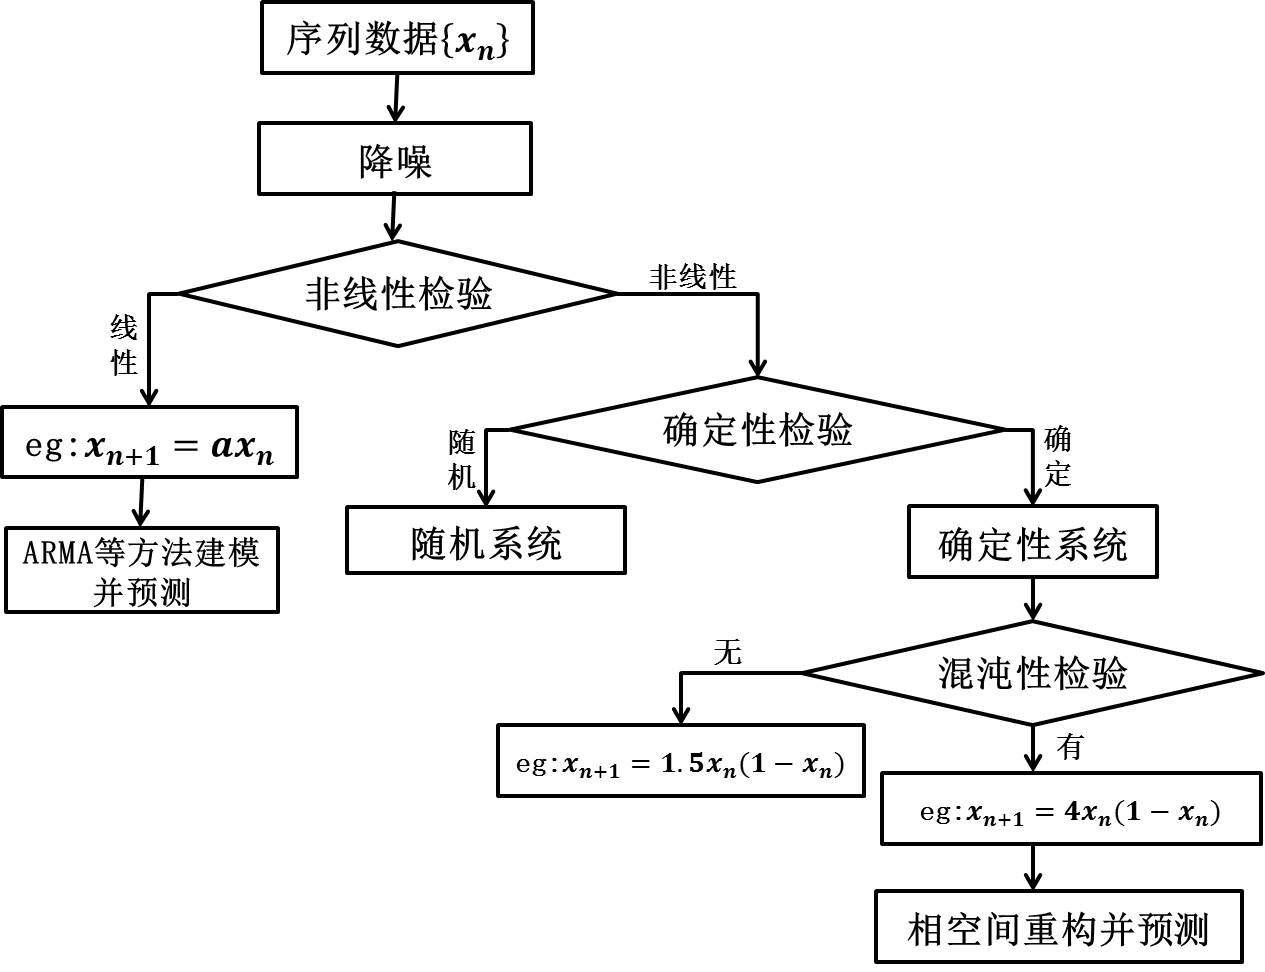
\includegraphics[height=8cm]{images/Time_series_modeling.jpg}
        \caption{时间序列建模流程图}
        \label{fig:时间序列建模流程图}
        \end{figure}
            % \textcolor[rgb]{1.00,0.00,0.00}{todo:图片:时间序列建模流程图}
            \par
            从上面的建模流程图中,可以看到,我们需要的工具有:序列降噪方法、非线性检验、平稳时间序列建模、确定性检验、混沌性检验、相空间重构以及预测方法。前面主要介绍的就是混沌系统的相空间重构以及混沌性检验方法,下面,我们来介绍非线性检验和确定性检验两种技术,关于序列降噪方法和平稳时间序列建模(ARMA等方法),在后面的数学建模实战部分会有一定的介绍。
        \subsubsection{非线性检验}
            \par
            常见的非线性检验方法有:AAFT、IAAFT、CAATT和GCR。下面,我们就来介绍基于替代数据思想的GCR方法。
            \par
            我们的目标是检验数据来自线性系统还是非线性系统,一种非常好的方法就是替代数据法。替代数据的基本思想是:原假设H0:$\{x_n\}_{n = 1}^N$来自某线性系统族。如果在这个H0的基础上,数据所表现出来的性质与线性系统相违背,那么,就可以拒绝原假设H0。我们从线性系统族中生成一些替代数据,如生成$M$个时间序列$\{\tilde{x}\}_i$,$i = 1,\dots ,M$,计算$M$个时间序列的统计量$Q_i,(i= 1,\dots ,M)$,统计量是样本的函数,可以是L指数、关联维度和Takens统计量,这之后在计算测量数据$\{x_n\}_{n = 1}^N$的统计量$Q_0$。最后,判断$Q_0$是否在$Q_i,(i= 1,\dots ,M)$的分布当中。
            \par
            上面的替代数据的思想正是假设检验的思想:在原假设H0成立时,$Q$统计量应该是什么样的分布(上面采用生成数据$\{\tilde{x}\}_i$,$i = 1,\dots ,M$来计算),而样本的实际统计量为$Q_0$,判断$Q_0$是否落在$Q$分布的拒绝域内。我们要讨论的是:如何从线性系统族中生成一些替代数据?
            \par
            下面,我们来讨论如何生成$M$个时间序列$\{\tilde{x}\}_i$,$i = 1,\dots ,M$。如果我们要求$\{\tilde{x}_n\}_i$与$\{x_n\}$来自同一分布,并且有近似的自相关性,我们可以考虑就在原序列$\{x_n\}$的基础上,值不变,打乱顺序即可生成$M$个时间序列$\{\tilde{x}_n\}_i$,这样$\{\tilde{x}\}_i$来自同一分布。然而,如何才能使$\{\tilde{x}_n\}$与$\{x_n\}$的自相关性相同呢?我们可以将这一要求转化为目标,利用前面介绍的GA等智能优化算法的思想,生成多个$\{\tilde{x}_n\}$,计算它们的自相关性,进化那些自相关性与$\{x_n\}$弱的样本$\{\tilde{x}_n\}$。
            \begin{align*}
                \min_\alpha \  \max\{|\tilde{C}(\tau) - C(\tau)|\}
            \end{align*}
            其中:$\alpha$为序列$\{x_n\}$的一种排列方式,例如$1,2,3...$和$3,2,4,...$。$\tilde{C}(\tau)$为样本$\{\tilde{x}_n\}$在$\tau$下的相关函数值,$C(\tau)$为样本$\{x_n\}$在$\tau$下的相关函数值。
            \par
            当然,在其它文献当中,可能定义$\max\{|\tilde{C}(\tau) - C(\tau)|\}$,$\tau = 1,2,\dots, \tau_{max}$为成本函数(损失函数),这也未尝不可。关于上面的$\min\max$问题的求解,利用GA等算法是简单的,但是在$\{x_n\}$的$n$较大时,要考虑计算量的问题。
            \par
            对于前面介绍的替代数据法,还存留一个问题,那就是检验统计量$Q$的选取及检验。$Q$一般选取L指数、关联维度$d$和K熵等系统的几何特征。也可以选取平均意义下的一步预测误差等。
            \par
            关于检验统计量$Q$的分布,我们有
            \[
                \frac{|Q_0 - \bar{Q}_s|}{\sigma_s} \ \dot{\sim}\  N(0,1)
            \]
            其中:$Q_0$为原序列$\{x_n\}$的检验统计量值,$\bar{Q}_s$为$M$个替代时间序列$\{\tilde{x}_n\}$的统计量平均值,$\sigma_s$为统计量方差。上面的分布渐进服从标准正态分布。

        \subsubsection{确定性检验}
            \par
            如果系统的将来值可以由过去值完全确定,则称系统为确定性系统,例如:$x_{n+1} = 4x_n$。我们可以写出确定性系统的一般形式
            \[
                x_{n+1} = F(x_n)
            \]
            这里的传递函数$F$完全已知。但是当确定性系统具有混沌特性时,一个小的测量误差会导致预测误差的极大变化,导致系统的不可测性。虽然不可测,但是混沌系统与随机系统仍是不同的,因为随机系统的未来值是完全不可预测的。对此,我们可以这样来做:设系统的观测序列为$\{x_n\}_{n = 1}^{N+l}$,用前$N$个观测值来重构相空间,并预测后$l$个值,记为$\{\hat{x}_n\}_N^{N+l}$,将其与$\{x_n\}_N^{N+l}$比较,然后设定判别规则。
            \par
            当然,关于预测问题,在1步预测时,如果认为1次预测有太大的随机性,也可以进行多次一步预测,然后取多次预测的平均值作为最终预测值。在多步预测时,有两种方案:\ding{172}利用BP等方法一次进行多步预测;\ding{173}一步一步的预测:将前一步预测值作为已知值,重构相空间,然后进行1步预测。
            \par
            王海燕的《非线性时间序列分析》一书中还提到过用递归图来判定系统的确定性。下面,我们直接介绍递归图的画法以及如何判断系统的确定性。
            \par
            设观测序列为$\{x_n\}_{n = 1}^{N+l}$,在$m,\tau$给定之后,重构相空间为$\Phi = \{\mathbf{x}_n\}_{n = N_0}^N$,相点$\mathbf{x}_n \in R^m$为系统在$n$时刻的状态。计算$i,j$时刻相点$\mathbf{x}_i,\mathbf{x}_j$的距离$d_{ij} = ||\mathbf{x}_i - \mathbf{x}_j||$,设定距离的阈值为$r$,以$i$为横坐标,以$j$为纵坐标,当$d_{ij}<r$时,在$(i,j)$处画一个点。观察递归图的对角线两侧是否有与对角线近似平行的小短线,如果有,则为混沌系统(确定性系统);如果没有,则为随机系统。注意:上面方法中的量和关联积分中的是相似的。

        \subsubsection{预测方法}
            \paragraph{零阶局部预测}
            对于混沌时间序列(混沌系统),我们在相空间重构的基础上来尝试的进行预测。对于原序列$\{x_n\}_{n = 1}^{N}$我们要预测其下一个状态值$x_{N+1}$,那么,在相空间重构上,预测$x_{N+1}$就相当于预测相点$\mathbf{x}_{N+1}$(相点$\mathbf{x}_{N+1}$中只有最后一个分量$x_{N+1}$是未知的)。现在,共有$N - N_0$个相点$\mathbf{x}_n \in R^m$,我们要根据这些相点预测下一个$\mathbf{x}_{N+1}$。基本思路是:相点$\mathbf{x}(N)$靠近$\mathbf{x} (N+1)$,我们在相空间$\Phi$中找到$k$个与$\mathbf{x}(N)$靠近的点$\mathbf{x}(N_1),\mathbf{x}(N_2),\dots,\mathbf{x}(N_k)$,那么,$\mathbf{x}(N_1+1),\mathbf{x}(N_2+1),\dots,\mathbf{x}(N_k+1)$这$k$个相点也靠近$\mathbf{x} (N+1)$,于是,我们可以让$k$个相点的平均值作为$\mathbf{x} (N+1)$的估计值
            \[
                \hat{\mathbf{x}} (N+1) = \frac{1}{k} \sum_{i = 1}^k \mathbf{x}(N_i+1)
            \]
            上述方法称为零阶局部预测。
            \paragraph{加权零阶局部预测}
            但是,不得不考虑$k$个相点与$\mathbf{x}(N)$接近的程度,这样,就可以设置加权零阶局部预测,让接近程度大的相点的权重大。用$d_i$表示$\mathbf{x}(N_i)$与$\mathbf{x}(N)$之间的距离,并令$d_{min} = \min \{d_i\}$,则加权零阶局部预测为
            \begin{align*}
                \hat{\mathbf{x}} (N+1) &=\frac{\sum_{i = 1}^k \mathbf{x}(N_i+1) e^{-l(d_i - d_{min})}}{\sum_{i = 1}^k e^{-l(d_i - d_{min})}}\\
                & =\sum_{i = 1}^k \frac{e^{-l(d_i - d_{min})}}{\sum_{i = 1}^k e^{-l(d_i - d_{min})}} \mathbf{x}(N_i+1)
            \end{align*}
            其中:$l$为外来参数,具有主观性;权重为
            \[
                w_N^i = \frac{e^{-l(d_i - d_{min})}}{\sum_{i = 1}^k e^{-l(d_i - d_{min})}}
            \]
            \par
            可以尝试着用局部回归核函数来替代权重,也可以用小波核来代替。由于参数$l$具有主观性,向晓东等人提出使用
            \[
                w_N^i = \frac{\frac{d_M - d_i}{d_M - d_{min}}}{\sum_{i = 1}^k \frac{d_M - d_i}{d_M - d_{min}}}
            \]
            来作为权重。
            \paragraph{加权1阶局部预测}
            像局部常数核权重回归和局部多项式核权重回归那样,对于零阶局部预测,我们有1阶局部预测和多阶局部预测,下面,我们来看一下加权1阶局部预测。
            \par
            前面,我们直接用$\mathbf{x}(N)$来替代$\mathbf{x}(N+1)$,现在,假设$\mathbf{x}(N+1)$与$\mathbf{x}(N)$之间是多项式关系,姑且先假设为1阶多项式(即线性),则有
            \[
                \mathbf{x}(N+1) = a+b\mathbf{x}(N)
            \]
            那么,接下来的工作就是求参数$a,b$。在相空间$\Phi$中找到$k,(k>m+1)$个与$\mathbf{x}(N)$邻近的相点$\mathbf{x}(N_1),\mathbf{x}(N_2),\dots,\mathbf{x}(N_k)$,则有
            \[
                a + b\vec{\mathbf{x}}(N_i) = \vec{\mathbf{x}}(N_i+1)
            \]
            其中:$\vec{\mathbf{x}}(N_i) = (\mathbf{x}(N_1),\mathbf{x}(N_2),\dots,\mathbf{x}(N_k)) ^{\mathrm{T}}$。\\
            于是,我们利用(加权)OLS等方法可以求解$a,b$
            \[
                a^*,b^* = \arg \min_{a,b} \ \sum_{i = 1}^k w_i [\mathbf{x}(N_i+1) - a - b\mathbf{x}(N_i)]^2
            \]
            最终,我们有
            \[
                \hat{\mathbf{x}}(N+1) = a^* + b^* \mathbf{x}(N)
            \]
            \paragraph{基于最大L指数的预测}
            假设相空间$\Phi$的最大L指数为$\lambda_1 $,找到相点$\mathbf{x}(N)$的最邻近点$\mathbf{x}(N\eta)$以及$\mathbf{x}(N\eta + 1)$,由最大L指数的物理意义
            \[
                e^{\lambda_1} = \frac{||\mathbf{x}(N+1) - \mathbf{x}(N\eta +1)||}{||\mathbf{x}(N) - \mathbf{x}(N\eta)||}
            \]
            有
            \[
                ||\mathbf{x}(N+1) - \mathbf{x}(N\eta +1)|| = d e^{\lambda_1}
            \]
            由于$\mathbf{x}(N+1)$中只有最后一个分量$x_{N+1}$是未知的,因此上式可解。

% \end{document}
